\chapter{Jet velocity from knot locations and radial oscillations}\label{chapter5}
%\doublespacing

%\textbf{(b)} Zoom-in of the top rectangular region in a) showing the bright knots in the northern jet. Contours are at 1.5, 2.7, 3.7, 5.1, 6.3, 7.5, 8.8, 10, 21, 37, 51, 72, 90, 103, 154, 311, and 466 mJy arcsec$^{-2}$. \textbf{(c)} Zoom-in of the bottom rectangular region in a) showing the bright knots in the southern jet. Contours are at 1.5, 2.0, 2.2, 2.7, 3.7, 5.1, 5.5, 6.0, 6.3, 6.8, 7.5, 8.8, 10, 21, 37, 51,  72, 90, 103, 154, 311, and 466 mJy arcsec$^{-2}$.

When I finished my modelling of the Hydra A northern jet based on the data presented in \citet{taylor90} (where only one knot is evident within the central 10~kpc, see Fig.~\ref{taylor}) I requested Professor Gregory Taylor to provide the original 6~cm VLA data, which I could use to study the jets near the core region more carefully and to estimate the brightness ratio of the jets. Studying the original data I realised that a fainter knot is apparent at approximately 3.7~kpc from the core in the northern jet. Therefore, a revision of the parameter space study was required in order to model both of these internal jet knots inside 10~kpc. In this section, I present my study of 2D axisymmetric jet-ICM interactions focusing on the two inner jet knots in the Hydra A northern jet. Fig.~\ref{northern} shows two bright knots marked by arrows, location of the shocks marked by $\times$, and the location of the turbulent transition of the jet to a plume marked by an arrow. 
\begin{figure}
\centering
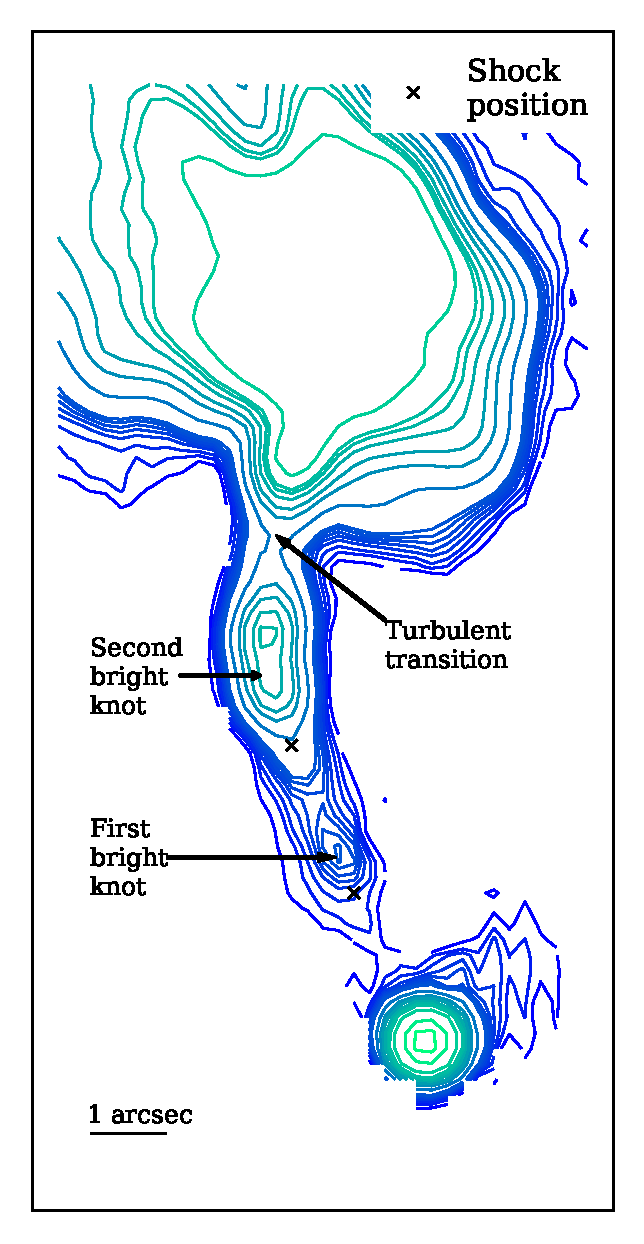
\includegraphics[width=5cm]{norhtern.eps}
\caption{Radio intensity map of the central 20~kpc region of the Hydra~A northern jet at 4.635 GHz. Contour levels are at 1.5, 2.7, 3.7, 5.1, 6.3, 7.5, 8.8, 10, 21, 37, 51, 72, 90, 103, 154, 311, and 466 mJy arcsec$^{-2}$. Two bright knots and the turbulent transition of the jet to a plume are marked by arrows. The location of the reconfinement shocks which we interpret as the cause of bright knots are marked by $\times$. }
\label{northern}
\end{figure}
%Hence, I repeated the previous parameter space study incorporating two inner knots.
Apart from incorporating two bright knots inside 10~kpc of the northern jet, I improve the axisymmetric model presented in the previous chapter with two additional features:

\paragraph{Conical opening jet:} In the numerical study of AGN jets, jets are considered to be either initially parallel \citep{sutherland07, wagner11} or initially conical \citep{komissarov98,krause12}. In the study of global effects of the jet-ambient medium interaction, for example, the mass or energy transport by the jet, it is not important whether the jet is initially parallel or conical. However, structures such as reconfinement shocks along the jet axis, are sensitive to the initial jet radius and the opening angle of the jet. Moreover, the fact that AGN jets are emitted from the black hole implies that they are initially expanding. For instance, the VLBI pc scale data \citep{taylor96} and VLA kpc scale data \citep{taylor90} of the Hydra A indicate that the jets expand from approximately 1~pc to approximately 200~pc. Therefore, for the modelling of jet structures near the core, a conical opening jet is more realistic. In the models presented in this chapter I use initially conical jet model following \citet{komissarov98}. 

\paragraph{Oscillatory nature of the jet boundary:} Oscillation of the jet boundary is a natural consequence of periodic reconfinement shocks \citep{prandtl1907, sanders83}. From the deconvolved FWHM of the jets of Hydra A \citep{taylor90}, a radial oscillation is apparent (see Fig. 6 of \citet{taylor90} and Fig.~\ref{f:radius} in this chapter). I did not consider the radial oscillation in the study presented in chapter~\ref{chapter4}. In this chapter, I consider both the knot locations and the oscillation of the jet boundary in modelling the northern jet.
%I started my study of the radio jets of Hydra A and its interaction with the cluster environment focussing the bright knot at approximately 3.7 and 7~kpc (deprojected) from the core. As explained in Chapter~\ref{introduction} and \ref{chap2} my proposal is that these two bright knots are a consequence of biconical shocks produced by the interaction of an over pressured jet with the cluster environment. 

Here I present a model of conically expanding jet entering the computational domain and interacting with the environment. I record the location of the shocks and the oscillation of the jet radius for a large number of models with different jet parameters. Both the shock locations and the oscillation of the jet boundary are used as fitting parameter to constrain the jet parameters, the jet radius $r_{\rm jet}$, the over-pressure ratio $p_{\rm jet}/p_{\rm a}$, the jet density parameter $\chi$ and the jet velocity $v_{\rm jet}$. The results are then analysed to obtain a best fit model for the Hydra A northern jet. The results of this study have been published in the journal MNRAS (Nawaz, M. A., Wagner, A. Y., Bicknell, G. V., Sutherland, R. S., and McNamara, B. R. 2014, MNRAS, 444, 1600).



%%%%%%%%%%%%%%%%%%%%%%%%%%%%%%%%%%%%%%%%%%%%%%%%%%%%%%%%%%%%%%%%%%%%%%%%
%
%												Description of Modelling
%
%%%%%%%%%%%%%%%%%%%%%%%%%%%%%%%%%%%%%%%%%%%%%%%%%%%%%%%%%%%%%%%%%%%%%%%%
\section{Jet parameters} \label{s:model}


 
\begin{figure}
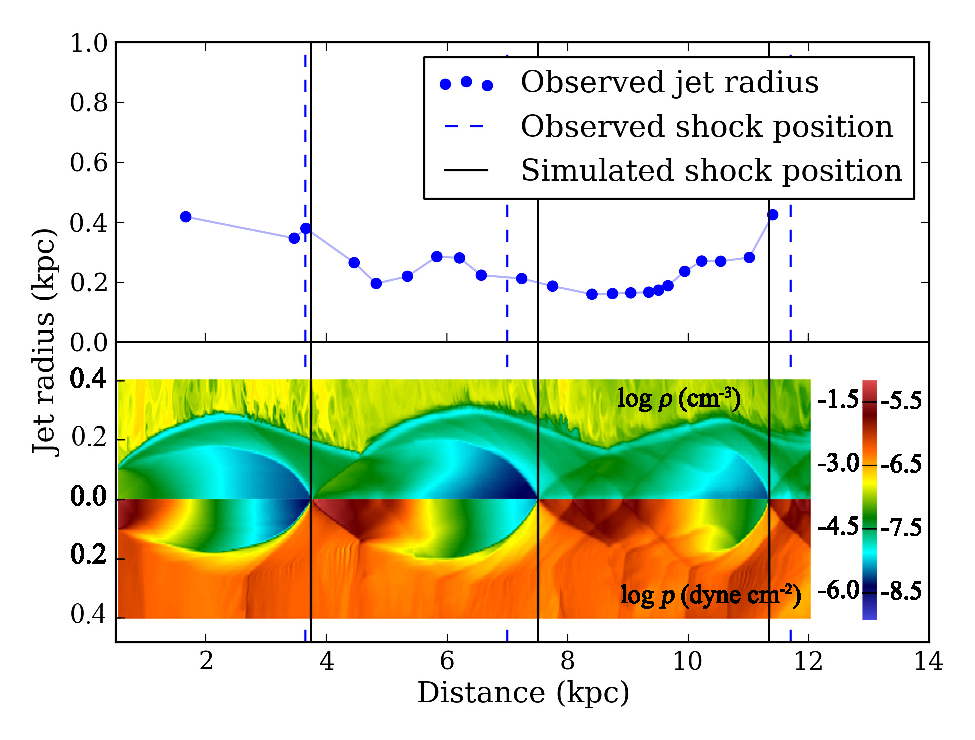
\includegraphics[width=\linewidth]{crp.eps}
\caption{Plot of the jet radius of the northern jet and the location of shocks as a function of the deprojected distance from the core. The radius is estimated from the deconvolved FWHM (see text). The vertical dashed lines represent the location of the southern edge of the first two bright knots in the northern jet, which correspond to the assumed locations of the shocks. In the bottom two panels the simulated logarithmic density and pressure slices show the periodically expanding and reconfining morphology and the shocks produced in the best-fit model for the northern jet. Both the radius plot and the images are stretched in the radial direction, emphasising the wave-like nature of the jet boundary. The vertical solid lines represent the shock positions in the simulations. The colourbar represents $\log \rho$ on the left and $\log p$ on the right.}
\label{f:radius}
\end{figure}


In this section I describe the selection of the initial jet parameters, the jet cross-sectional area $A_{\rm jet} = (\pi r_{\rm jet}^2$, where $r_{\rm jet}$ is the jet inlet radius), the jet pressure $p_{\rm jet}$, the jet density parameter $\chi = \rho_{\rm jet} c^2 / (\epsilon_{\rm jet} + p_{\rm jet})$, where $\rho_{\rm jet}$ and $\epsilon_{\rm jet}$ are the rest mass density and the energy density of the jet respectively and the jet Lorentz factor $\Gamma = (1- \beta^2)^{-1/2}$.  These parameters are assigned so as to be consistent with the expression for the jet power (equation~\ref{jet_power}).
%\begin{equation}
%P_{\rm{jet}} = \frac{\gamma}{\gamma -1} c p_{\rm{jet}}\Gamma^2\beta A_\mathrm{jet}\left(1+\frac{\Gamma -1}{\Gamma}\chi\right)\:.
%\label{jet_power}
%\end{equation} 
%\citep{sutherland07a}


\subsection{Magnetic field}\label{s:mag}	


In the simulations I neglect the magnetic field. Is this a reasonable approximation given the popular notion that jets may be collimated by the toroidal field, which develops as a result of the rotation of the flow ejected from the accretion disk \citep{blandford82a} or from the ergosphere \citep{blandford77a}? In this case one expects the magnetic and particle pressures to be comparable. Moreover, this would argue against the assumption of invoking an over-pressured jet on the parsec-scale (see below). Self-collimation by a toroidal magnetic field is an appealing mechanism for the region of jets just outside the Alfven surface. However, the fact that the jet expands by a factor of over 200 between the parsec scale and the kiloparsec scale indicates that self-collimation does not occur in this region. For example the self-similar models of \citet{li92a} and \citet{vlahakis03a} indicate that asymptotically the flow becomes cylindrical when the jet is magnetically collimated. A different model has been proposed by \citet{spruit11a}, who has argued that three-dimensional effects lead to reconnection of the magnetic field and that the loss of magnetic energy produces a pressure gradient, which is responsible for the acceleration of jets to high Lorentz factors. \citet{moll09a,moll10a} has carried out numerical simulations based on this concept, in the context of protostellar jets. There is also observational support for 
sub-equipartition magnetic fields on the sub-parsec scale in a substantial fraction of gamma ray blazars. In a recent paper \citet{zhang14a} modelled the spectral energy distributions of a number of BL~Lac objects and flat spectrum radio quasars (FSRQs) and found that they divide along the line magnetic~power = electron~power with most of the BL~Lac objects being below this dividing line (see their Fig. 13(b)). The respective powers are proportional to the energy densities of the various components (their section 4) so that the ratio of the magnetic power to electron power informs us of the ratio of the respective energy densities. Hence, the magnetic energy densities in many of the BL~Lac objects are well below the electron energy density (but with some members of the sample approaching equality). Thus there is good justification, in the first instance, for neglecting the magnetic field with the implication that the beamed counterpart of Hydra~A would be a BL~Lac object rather than a quasar. 

 
What values of the jet density parameter, $\chi$ are relevant in this context? Two main options for jet composition are generally discussed -- electron-positron or electron-proton. Let $m_e$ be the electron mass and $m_+$ the mass of the positively charged component, $m_e$ for a positron and $m_p$ for a proton. The parameter $\chi$ is then given by: 
\begin{equation}
\chi = 0.75(a-2)(a-1)^{-1} \, \frac {m_+}{m_e} \gamma_1^{-1},
\end{equation}
where $a$ and $\gamma_1$ are defined in \S~\ref{s:powr}. Note that, for an electron positron jet with $a=2.4$ and $\gamma_1 \gtrsim 10$, $\chi \ll 1$. The theory of jet production from black holes \citep{blandford77a} and X-ray observations of the lobes of both FR1 and FR2 radio galaxies \citep{croston05a,croston14} make the concept of electron-positron jets appealing. However, the issue of jet composition is by no means settled. In an electron-proton jet, low values of $\chi$ require the low energy cutoff, $\gamma_1 \gg 1$. 


\subsection{Over-pressured jets}\label{s:opj}

A key feature of the jet model is that the bright knots beginning at $\sim3.7$ and 7.0 and 11.0 kpc from the core in the northern jet and at $\sim 2.5$, 3.9, 5.4 and 6.7 kpc in the southern jet are the result of  consecutive biconical shocks following recollimation of over-pressured jets. I have identified the points where the surface brightness gradient markedly increases, as the location of the upstream side of each knot (See Fig.~\ref{northern} and Fig.~\ref{southern}). The third knot in the northern jet occurs just as the jet merges into the lobe so that I might expect the location of this knot to be affected somewhat by the jet's transition to turbulence.  

\citet{norman82} first drew attention to the production of biconical and normal shocks (Mach discs) in over-pressured astrophysical jets. An initially over-pressured jet expands laterally and its thermal pressure and ram pressure decreases with distance along the direction of propagation. When the jet pressure reaches the ambient pressure the jet begins to recollimate. The jet periodically expands and recollimates, producing a series of biconical or normal shocks along the jet axis. This phenomenon had been known to laboratory hydrodynamicists for some time and \citet{birkhoff57a} associated it with the \emph{natural wavelength} of a supersonic jet $\Lambda$ (see equation~\ref{e:birkhoff}). 

It is feasible that the Hydra A jets are initially over-pressured since the minimum energy pressure in the pc-scale northern jet, 27 pc from the central black hole \citep{taylor96} is $1.33\times10^{-7}$ and $1.26\times10^{-7} \rm \ dynes \ cm^{-2}$ for $\beta=0.2$ and 0.9 respectively. (A jet diameter of 26 pc was used in these estimates). These minimum energy pressure estimates are about a factor of 200 times higher than the central pressure $\approx 6.6\times10^{-10} \rm \ dynes \ cm^{-2}$ of the modelled interstellar medium (see \S~\ref{s:cluster}). Moreover, using these pressures underestimates the jet kinetic power at $ \approx 2.4 \times10^{44} \ \rm erg \ s^{-1}$ for $\beta =0.8$ and $\chi \sim 10^{-2}$ compared to the value $10^{45} \ \rm erg \ s^{-1}$ used in the models by a factor $\approx 4$. Therefore the value of the jet kinetic power of the models implies a jet pressure $6~\times p_{\rm min} \approx 7.0 \times 10^{-7} \rm \ dynes \ cm^{-2} $ at 27~pc. This is approximately 100 times the central atmosphere pressure. If I assume that the jet expands adiabatically, i.e., the jet pressure decreases with the jet radius according to $p_{\rm jet}\propto r_{\rm jet}^{-8/3}$, I obtain an over pressured jet $5~p_{\rm a}$ at 0.5~kpc  from the core (where I initialise the jet in the computational domain) with a jet radius 100 pc. 


Interpreting the jet as over-pressured on the parsec scale implies that from the parsec to the kiloparsec scale it is freely expanding. I also note here that, in a detailed analysis of protostellar jets \citet{cabrit07a} has concluded that those jets are initially magnetically collimated but are freely expanding at some distance ($\sim 50 \> \rm AU$) from the star. Of course, these scales are not directly commensurable with Hydra~A, but a long held view is that the physics of protostellar and AGN outflows are similar in many respects.


The proposition of the jet bright knots as biconical shocks is further reinforced by the observed wave-like nature of the northern jet boundary. Fig~\ref{f:radius} shows the radius profile (dots) of the northern jet, which I obtain by assuming the jet as a homogeneous cylinder and utilising the deconvolved FWHM of the jet \citep{taylor90} $\Phi_{\rm jet}$ together with $r_{\rm jet} = \Phi_{\rm jet}/ \sqrt{3}$. In order to illustrate the association of biconical shocks with the sinusoidal radius profile I attach the logarithmic density and pressure images (panels marked with $\log\rho$ and $\log p$ respectively) of one of the best fit models Ciii for the northern jet. In the simulated radius profile I see the jet boundary oscillates and at $\sim 0.7 \ \rm kpc$ before each radius minimum biconical shocks appear. These are clearly indicated by the large increase in pressure. The observed and simulated shock locations are marked with dashed and solid vertical lines respectively.

I construct models of the northern jet for which data on the jet FWHM are more complete. The modelling strategy for this jet is as follows. I conduct a parameter space study searching for numerical models which can successfully reproduce the correct shock locations and the radius profile of this jet. 

In the axisymmetric numerical models of the jet-ICM interaction I deal with straight jets whereas the Hydra A jets are curved. However since the curvature of the jets are modest within the central 10~kpc, I expect an approximation by a straight jet to be reasonable.

As stated above, in order to model the jets of Hydra A I require five jet parameters, the jet kinetic power $P_{\rm{jet}}$, the initial jet radius $r_{\rm{jet}}$, the initial jet pressure $p_{\rm{jet}}$, the initial jet velocity $\beta$ (in units of the speed of light), and the jet density parameter $\chi$, of which four are independent. In the previous section I established a value for the jet kinetic power $10^{45} \rm erg \ s^{-1}$. In the following I describe how I choose the other three independent jet parameters and set their values. 

The first parameter is the jet kinetic power, which is reasonably well-determined by the radio and X-ray observations. The jet radius is the second parameter; this affects the downstream scale of the oscillating jet boundary and is not known \emph{ab initio}. The third parameter is the jet pressure ratio; this affects both the amplitude of the radial oscillations and the knot spacing. The fourth parameter is the jet velocity, $\beta$. Then the parameter $\chi$ is determined using equation~\ref{chi2}.
%by solving equation~(\ref{jet_power}) for $\chi$, that is,
%\begin{equation}
%\chi = \frac{\Gamma}{\Gamma -1}\left( \frac{\gamma-1}{\gamma}\frac{P_{\rm{jet}}}{c p_{\rm{jet}} \Gamma^2\beta A_{\rm{jet}}} -1 \right)\:.
%\label{chi2}
%\end{equation}

Referring to the expression for the natural wavelength $\Lambda$ of a supersonic \emph{non-relativistic} jet in near pressure equilibrium $\Lambda/r_{\rm jet} \approx 2.6 \sqrt{M^2 - 1}$
% \begin{equation}
%\Lambda/r_{\rm jet} \approx 2.6 \sqrt{M^2 - 1}
%\label{e:birkhoff}
%\end{equation}
\citep{birkhoff57a}, I note that the selection of the velocity and density parameters is equivalent to defining the Mach number, 
\begin{equation}
M = (2+3 \chi)^{1/2} \Gamma \beta
\end{equation} 
\citep{bicknell94a}. 
%$=(2+3 \chi)^{1/2} \Gamma \beta$ \citep{bicknell94a}. 

Following \citet{komissarov98} and \citet{krause12} I model the jet as ballistic and conically expanding in the first 
0.5~kpc, which represents the base of the computational domain. \citet{komissarov98} used an identical setup in their simulations to show that an initially conical jet may be collimated by the ambient pressure. \citet{krause12} performed simulations, also with identical initial conditions to provide a theoretical basis for the FRI/FRII classification of radio sources based on the half cone angle of the initial jet cone.

To summarize, I set up my simulations with an initially over-pressured (in one case equilibrium pressure) conically expanding jet with cross-sectional radius $r_{\rm{jet}}$ and centre at $(r, z) = (0, 0.5)$ kpc, where $r$, and $z$ are the radial and height coordinate of the axisymmetric cylindrical domain.  The independent jet parameters are jet power $P_{\rm{jet}}=10^{45}\,\rm erg \, s^{-1}$, jet radius $r_{\rm{jet}}$, inlet jet pressure $p_{\rm{jet}}$, inlet jet velocity $\beta$. The remaining jet parameter $\chi$ is determined from Eqn.~\ref{chi2}
The components of the jet velocity at a points $(r, z)$ within the initial conically expanding jet cross-section are $v_r = \beta z/\sqrt{r^2 + z^2}$ and $v_z =\beta r/\sqrt{r^2 + z^2}$. 


%%%%%%%%%%%%%%%%%%%%%%%%%%%%%%%%%%%%%%%%%%%%%%%%%%%%%%%%%%%%%%%%%%%%%%%%
%
%												CODE AND SIMULATION PARAMETERS
%
%%%%%%%%%%%%%%%%%%%%%%%%%%%%%%%%%%%%%%%%%%%%%%%%%%%%%%%%%%%%%%%%%%%%%%%%
\section{Grid of models} \label{s:code}

%% TBD Fix table with new values of n_e (done)

%\begin{table*}
\begin{sidewaystable}[htbf]
\caption{Simulation parameters. In all simulations, $P_{\rm{jet}}=10^{45} \rm \ erg \ s^{-1}$.}
\centering
\begin{tabular}{l * {9}{c}}
\hline \hline
Model  & $r_{\rm{jet}}(pc)$ & $p_{\rm{jet}}/p_{\rm{a}}$ & $\beta$ & $\chi$ & $\eta$ & $\phi$ (rad cm$^{-2}$) & $\Psi_{6\rm{cm}}$ (rad) & $\Psi_{20\rm{cm}}$ (rad) \\
\hline
    %%%%%%%%%% 		set A 	%%%%%%%%%%%%%%%
%	\multicolumn{9}{c}{Set A, $r_{\rm{jet}}=0.18 \rm \ kpc$} \\ 
	\hline
	 Ai    &  180 &   2  &  0.40  &     251.19 &   5.62$\times10^{-3}$  &    4.95$\times10^{-4}$         &     1.78$\times10^{-2}$		&  1.98$\times10^{-1}$      \\	 
  	 Aii 	& 180 &  	2  &  0.70 & 	23.17 &	 5.18$\times10^{-4}$ & 	4.56$\times10^{-5}$ 	&	1.64$\times10^{-3}$		&  1.83$\times10^{-2}$	  \\
	 Aiii 	& 180 &  	2  &  0.75 & 	15.03 &	 3.37$\times10^{-4}$ &	2.97$\times10^{-5}$ 	&	1.07$\times10^{-3}$		&  1.19$\times10^{-2}$	  \\
	Aiv 	& 180 & 	2  & 	0.80 & 	9.27   &  	2.07$\times10^{-4}$  &	1.83$\times10^{-5}$		&	6.57$\times10^{-4}$ 	&  7.30$\times10^{-3}$	 \\
	Av 	& 180 & 	2  & 	0.85 & 	 5.10  & 	1.14$\times10^{-4}$ &	 1.01$\times10^{-5}$	& 	3.62$\times10^{-4}$		&  4.02$\times10^{-3}$  	 \\
	 Avi 	& 180 & 	2  &	0.90 &  	2.14   & 	4.79$\times10^{-5}$  &	 4.22$\times10^{-6}$	&  	1.52$\times10^{-4}$		&  1.69$\times10^{-3}$ 	\\
	 Avii  &  180  &  2  & 0.95  &   0.11  &   2.40$\times10^{-6}$       &    2.11$\times10^{-7}$		&	7.60$\times10^{-6}$		&   8.45$\times10^{-5}$  \\
		\hline
	  %%%%%%%%%% 		set  B	%%%%%%%%%%%%%%%
%	\multicolumn{9}{c}{Set B, $r_{\rm{jet}}=0.15 \rm \ kpc$} \\ 
        Bi    &  150  & 2  &  0.40  &   366.98  & 8.21$\times10^{-3}$  & 6.02$\times10^{-4}$ 	& 	2.17$\times10^{-2}$ 	& 	2.41$\times10^{-1}$  \\
  	 Bii 	& 150 &  2  &  0.70 &   34.90 & 7.80$\times10^{-4}$  &	5.73$\times10^{-5}$		&	2.06$\times10^{-3}$		&	2.29$\times10^{-2}$  \\
	 Biii 	& 150 &  2  &  0.75 &   23.00 & 5.14$\times10^{-4}$  &	3.78$\times10^{-5}$		&	1.36$\times10^{-3}$		&	1.51$\times10^{-2}$  \\
	Biv 	& 150 & 2  &  0.80 & 14.45   & 3.23$\times10^{-4}$   &	2.37$\times10^{-5}$		&	8.54$\times10^{-4}$ 	&  	9.49$\times10^{-3}$	 \\
	Bv 	& 150 & 2  &  0.85 &  8.28  & 1.85$\times10^{-4}$     &     1.36$\times10^{-5}$		&	4.89$\times10^{-4}$		&   	5.44$\times10^{-3}$	 \\
	Bvi 	& 150 & 2  &  0.90 & 3.87  &  8.64$\times10^{-4}$     &	6.34$\times10^{-6}$		&	2.28$\times10^{-4}$		& 	2.54$\times10^{-3}$ 	\\
	Bvii 	& 150 & 2  &  0.95  & 0.79 & 1.78$\times10^{-5}$	&    1.30$\times10^{-6}$		&      4.69$\times10^{-5}$		&      5.21$\times10^{-4}$   \\
 	Bviii    & 150 & 5 & 0.70 & 11.86  & 6.63$\times10^{-4}$      & 	4.87$\times10^{-5}$		& 	1.75$\times10^{-3}$		&      1.95$\times10^{-2}$   \\
	Bix    & 150 & 5 & 0.75 & 7.43   & 4.15$\times10^{-4}$      & 	3.05$\times10^{-5}$		&	1.10$\times10^{-3}$		&	1.22$\times10^{-2}$ \\
	Bx    & 150 & 5  & 0.80  &  4.28 & 2.39$\times10^{-4}$    &    1.76$\times10^{-5}$		&	 6.32$\times10^{-4}$	& 	7.02$\times10^{-3}$  	\\
	Bxi  & 150 & 5  &  0.85 &   2.04  &   1.14$\times10^{-4}$    &	8.39$\times10^{-6}$ 	&  	 3.02$\times10^{-4}$	&  	3.35$\times10^{-3}$ \\
        Bxii   &  150 & 5  &  0.90 &   0.48  &  2.70$\times10^{-5}$   &	1.98$\times10^{-6}$ 	&    	 7.13$\times10^{-5}$	&  	7.92$\times10^{-4}$	 \\
	\hline
	  %%%%%%%%%% 		set C 	%%%%%%%%%%%%%%%
%	\multicolumn{9}{c}{Set C, $r_{\rm{jet}}=0.10 \rm \ kpc$} \\
        Ci     &  100 & 5  & 0.40    &  329.08  & 1.84$\times10^{-2}$ &   9.00$\times10^{-4}$		&      3.24$\times10^{-2}$		&      3.60$\times10^{-1}$ \\
	Cii	& 100  & 5  & 0.70  & 31.06 & 1.74$\times10^{-3}$	  &   8.50$\times10^{-5}$		&	3.06$\times10^{-3}$		&	3.40$\times10^{-2}$ \\
	Ciii	& 100  & 5  & 0.75  & 20.41 & 1.14$\times10^{-3}$ 	  &   5.58$\times10^{-5}$	 	&      2.01$\times10^{-3}$		&	2.23$\times10^{-2}$ \\
  	Civ    & 100 &  5  & 0.80  & 12.75  &  7.83$\times10^{-4}$  &   3.49$\times10^{-5}$  	&	1.26$\times10^{-3}$ 	&  	1.40$\times10^{-2}$ 	\\
	Cv   & 100 &  5  &  0.85 &   7.24   &  4.45$\times10^{-4}$  &   1.98$\times10^{-5}$ 		&  	7.13$\times10^{-4}$		&      7.92$\times10^{-3}$  \\
	Cvi   & 100 & 5  &  0.90 &   3.30  &  2.03$\times10^{-4}$   &	9.03$\times10^{-6}$  	&  	 3.25$\times10^{-4}$	&       3.61$\times10^{-3}$	 \\
	Cvii   & 100 & 5 & 0.95  & 0.57  &  3.18$\times10^{-5}$	  &    1.56$\times10^{-6}$		&      5.61$\times10^{-5}$		&       6.33$\times10^{-4}$  \\
	Cviii  & 100 &  5  &  0.96  & 0.15  & 8.33$\times10^{-6}$	  &    4.08$\times10^{-7}$		&      1.47$\times10^{-5}$		&      1.63$\times10^{-4}$ \\
	\hline
	 Di 	& 120  & 5   &  0.50    & 96.96	  & 5.48$\times10^{-3}$	 & 	3.22$\times10^{-4}$ 	&	1.16$\times10^{-2}$		&  1.29$\times10^{-1}$	  \\
	 Dii 	& 100  & 5   &  0.50 & 144.34  & 8.07$\times10^{-3}$ &	3.95$\times10^{-4}$         &	1.42$\times10^{-2}$		&  1.58$\times10^{-1}$	  \\ 
	 Diii 	& 80    & 10   &  0.50  & 111.14  &  1.24$\times10^{-2}$    &	4.86$\times10^{-4}$		&	1.75$\times10^{-2}$ 	&  1.95$\times10^{-1}$	 \\
	 Div 	& 80    & 15   &  0.50  &  71.60 	  & 1.20$\times10^{-2}$     &	 4.70$\times10^{-4}$	& 	1.69$\times10^{-2}$		&  1.88$\times10^{-1}$  	 \\
	 Dv 	& 60    & 10   &  0.50  &  203.38  & 2.27$\times10^{-2}$     &	 6.68$\times10^{-4}$	&  	2.40$\times10^{-2}$		&  2.67$\times10^{-1}$ 	\\
	 Dvi 	& 60    & 15   &  0.50  &  133.10  & 2.23$\times10^{-2}$     &	 6.55$\times10^{-4}$	&  	2.36$\times10^{-2}$		&  2.62$\times10^{-1}$ 	\\
	 \hline
\end{tabular}
\label{t:sim_par}
\end{sidewaystable}
%\end{table*}



For my simulations I use the the publicly available PLUTO code \citep{mignone07} and produce two dimensional axisymmetric hydrodynamic models of the jet-ICM interaction in Hydra A. Since my  models involve relativistic velocities I use the relativistic hydrodynamic (RHD) module available in PLUTO. Detail description of the code and the problem initialisation are given in Chapter~\ref{chapter2}.

%The $(r, z)$ computational domain for the two dimensional axisymmetric simulations is a cylinder of radius $r=25$ kpc and height $z=50$ kpc. Using a stretched grid I define a high resolution grid within the central $10\,\mathrm{kpc}\times1\,\mathrm{kpc}$ region, giving us 10 cells across the jet inlet, and a lower resolution in the outer regions. I impose an axisymmetric boundary condition for the boundary $r=0$, and a reflective boundary condition for $z=0$.  The remaining boundaries are set to outflowing boundaries.
%
%I use the \citet{taub1948a} equation of state, a quadratic approximation to the exact Synge--J\"{u}ttner relativistic perfect gas equation of state \citep{juttner1911a,synge1957a}, which yields $\gamma\rightarrow5/3$ in the low temperature limit, and $\gamma\rightarrow4/3$ in the high temperature limit. 
%Because the radiative cooling time of the ambient gas and the synchrotron cooling time of the jet plasma are large compared to the simulation time, I do not include radiative cooling in my  simulations.
%
%The initial conditions for the ambient medium representing the hot ICM surrounding Hydra A are the hydrostatic thermodynamic profiles found in \S~\ref{s:cluster}. 

To determine the optimal values for the three initial jet parameters $r_{\rm{jet}}$, $p_{\rm{jet}}$, and $\beta$ for the Hydra A northern jet, I compare the radius profile of the jet and the locations and spacing of the reconfinement shocks in my  simulations with the observed radius profile and shock positions as indicated by the locations of the two bright knots. The thirty three sets of parameters that I have used are summarised in Table~\ref{t:sim_par}. I have not utilised every possible combination of parameters since I have restrictions on the jet radius minimum of 160 pc. I have not used models with five times over-pressured jet with jet inlet radius 180 pc and two times over-pressured jet with inlet radius 100 pc since they will produce much larger or smaller minimum in the radius profile than 160 pc. Since by experimenting models with lower jet velocities I obtain significantly large shock spacing compared to the observed shock spacing, I have not presented models with $\beta < 0.4$. A grid of models with jet $\beta = 0.5$ which exhibit larger shock spacings is presented in \S~\ref{s:b_r} 

For an additional check for the consistency of the jet parameters, some derived parameters, namely the density parameter $\chi$, the density ratio $\eta$ of the jet and the atmosphere at the jet base, the rotation measure (RM) $\phi$, and the Faraday rotation angle $\Psi$ at 6 cm ($\Psi_\mathrm{6cm}$) and 20 cm ($\Psi_\mathrm{20cm}$) are also summarised in Table \ref{t:sim_par}. Unlike models with a single knot (presented in chapter~\ref{chapter4}), all of the Faraday rotation values are comfortably less than unity and in the best models, Ciii, Civ and Cv, much less than unity.

%The rotation measure and Faraday rotation of the central jet with electron density $n_\mathrm{\mathrm e,jet}$(=$\rho_{\mathrm jet}$(1 + 2 $n_{\mathrm He}$/$n_{\mathrm H}$)/u(1 + 4$n_{\mathrm He}$/$n_{\mathrm H}$), where $u$ is an atomic mass unit), magnetic field along the line of sight $B_z$ (we use $35 \> \mu\,\mathrm{G}$, approximately the minimum energy magnetic field near the jet base), differential plasma depth $dl$, jet radius $R_{\rm{jet}}$, total plasma depth $L=2R_{\rm{jet}}$, and wavelength $\lambda$ are calculated from
%\begin{eqnarray}
%\phi &=& 8.1\int n_\mathrm{e,jet} B_z dl \quad \rm rad \, cm^{-2} \nonumber \\
%&=& 8.1\times10^{-5}\, \left(n_{e, jet}\right) \left(\frac{B_z}{\mathrm{\mu G}}\right)  \left(\frac{2R_{\rm{jet}}}{\mathrm{kpc}} \right) \rm rad \, cm^{-2}
%\end{eqnarray}
%where the units of $B_z$ and $l$ are Gauss and cm, respectively. The total Faraday rotation through the jet is given by:
%\begin{equation}
%\Psi_{\rm rad} = \phi \lambda^2 \:.
%\end{equation}

%I calculate these quantities as an additional check to ensure that the jet parameters are consistent with the observation that the radio emission along the length of the jet is polarized. The internal Faraday rotation should be much less than unity for consistency between the models and the observations. Note however, that the values given in Table~\ref{t:sim_par} are maximum values and do not take into account the angle between the magnetic field and the line of sight, the possibility that the magnetic field strength may be below equipartition, or the occurrence of field reversals. Nevertheless, all of the Faraday rotation values are comfortably less than unity and in the best models, Ciii, Civ and Cv, much less than unity.

I group the runs into four sets as set out in Table~\ref{t:sim_par}; Sets A, B and C correspond to simulations with initial jet radii of $0.18  \> \rm kpc$, $0.15 \> \rm kpc$ and $0.10 \> \rm kpc$, respectively. Set D corresponds to model with jet $\beta = 0.5$ and initial jet radii $0.12, \> 0.10, \> 0.08 \> \rm and \> 0.06 \> kpc$.   

%%%%%%%%%%%%%%%%%%%%%%%%%%%%%%%%%%%%%%%%%%%%%%%%%%%%%%%%%%%%%%%%%%%%%%%%
%
%									Simulation Results
%
%%%%%%%%%%%%%%%%%%%%%%%%%%%%%%%%%%%%%%%%%%%%%%%%%%%%%%%%%%%%%%%%%%%%%%%%

\section{Simulation Results}\label{s:sims}

In this section I present the results of my two-dimensional axisymmetric hydrodynamic simulations, including the parameter study described above. I have conducted a series of simulations to cover the parameter space described in 
Table~\ref{t:sim_par}. I first describe the results of my  parameter space study, which enable us to constrain the jet velocity and other jet parameters at 0.5 kpc from the black hole. These provide best fit models for the northern Hydra A jet. Using one of the best fit models, Civ, I then discuss the association of biconical shocks with the bright knots, the turbulent transition of the jet, and the flux density ratio between the northern and southern jet of Hydra A. Finally, based on the discrepancy between the simulated and the observed flux density ratio, I explore the possibility of varying the angle of inclination within the range defined by \citet{taylor93}. 

%%%%%%%%%%%%%%%%%%%%%%%%%%%%%%%%%%%%%%%%%%%%%%%%%%%%%%%%%%%%%%%%%%%%
%
%		PARAMETER STUDY
%
%%%%%%%%%%%%%%%%%%%%%%%%%%%%%%%%%%%%%%%%%%%%%%%%%%%%%%%%%%%%%%%%%%%%

\subsection{Parameter space study for the northern jet}\label{s:param_study}

The aim of the parameter space study is to obtain optimal values for the jet parameters, in particular, the jet radius, the jet pressure and the jet velocity at $0.5$ kpc from the core.

\begin{figure}
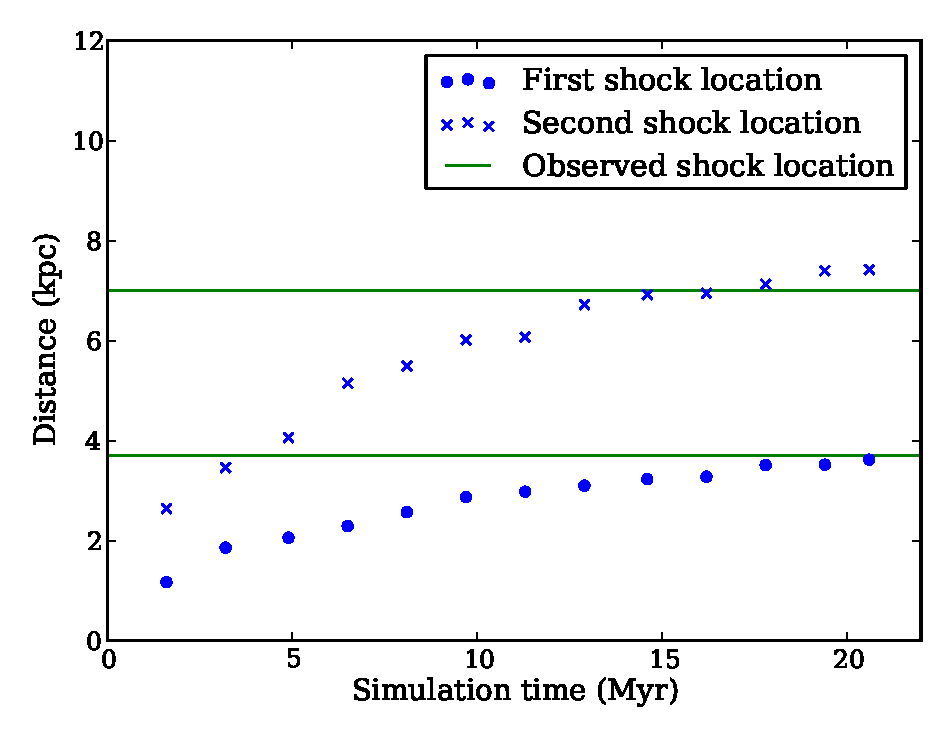
\includegraphics[width=\linewidth]{css.eps}
\caption{
Evolution of the locations of the first (blue dots) and second (blue crosses) shocks with time for run Civ. The horizontal lines represent the observed shock locations. This figure shows that the first two reconfinement shocks move downstream with time and asymptote towards  3.6 and 7.4 kpc at approximately 20 Myr. }
\label{f:s_ev}
\end{figure}

\begin{figure*}
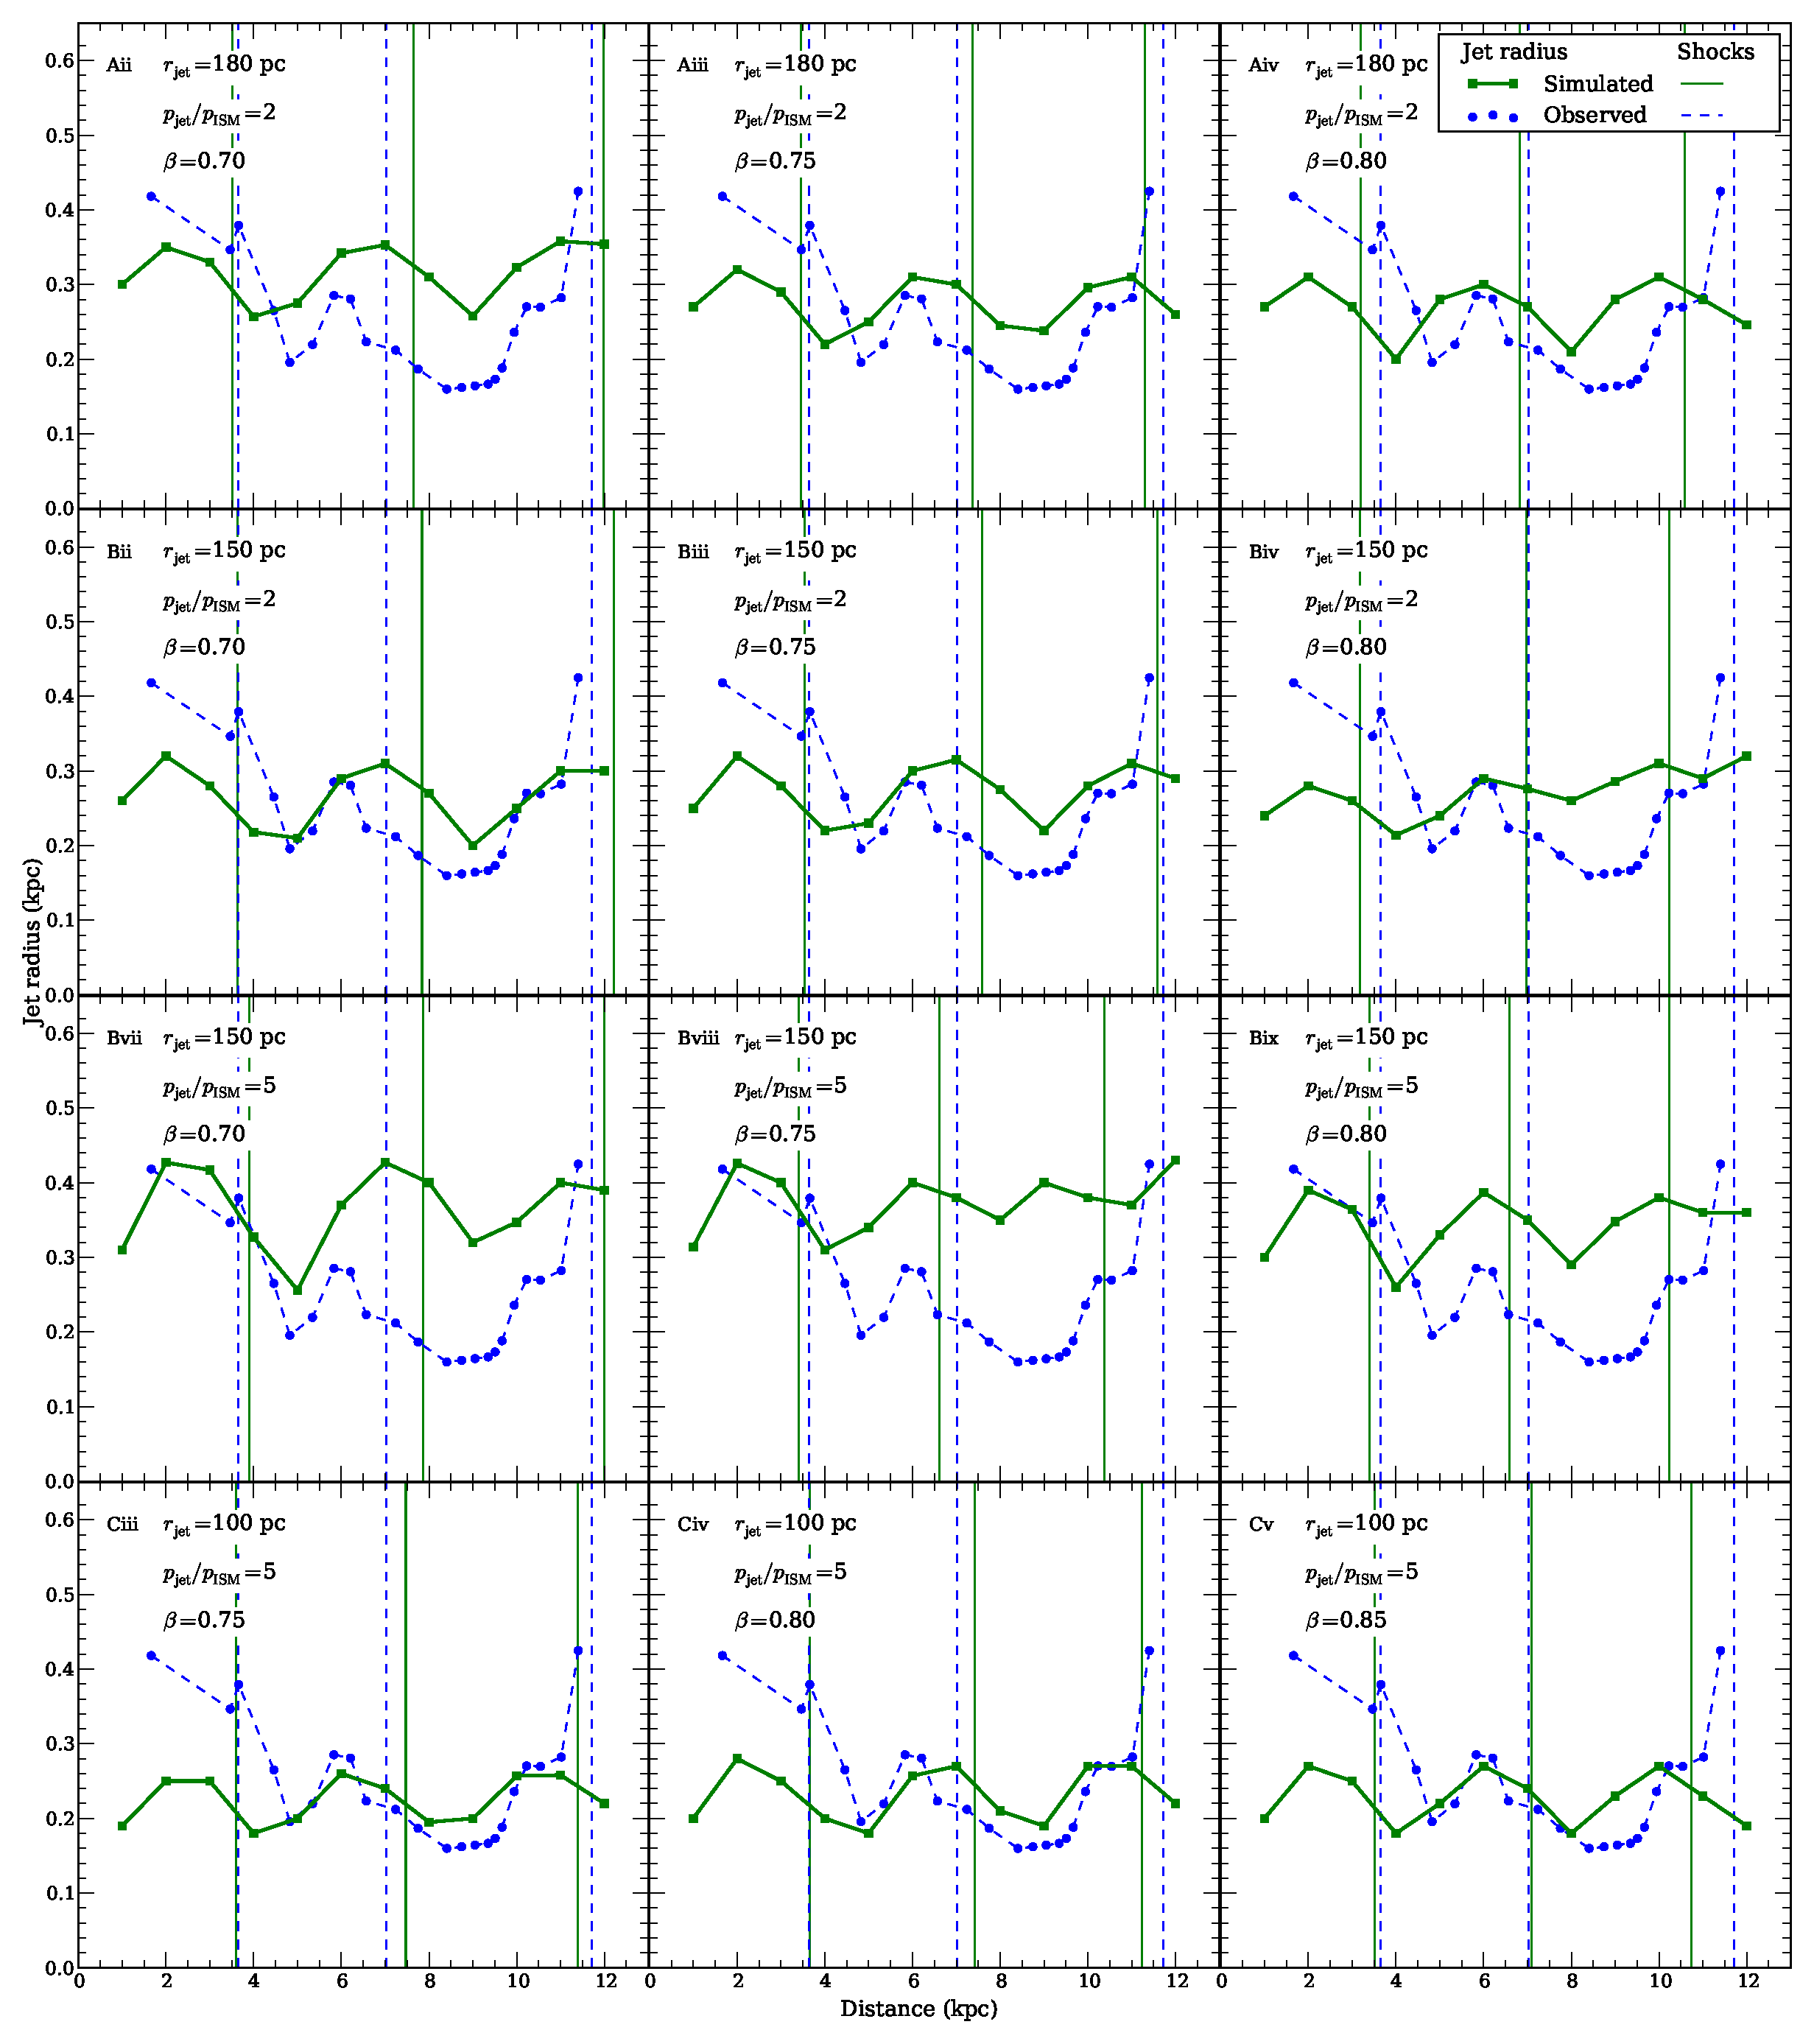
\includegraphics[width=\textwidth]{cmr.eps}
\caption{
Jet radius profiles and shock positions along the jet extracted from selected hydrodynamic simulations. The green line with squares, and the blue lines with circles represent simulated and observation data of radius, respectively. The blue dashed and green solid vertical lines represent the observed and simulated shock locations, respectively. The top row of panels are simulations from set A, the second and third rows of panels are simulations from set B, and the bottom row of panels are simulations from set C. In the simulations shown in the upper two rows of panels, $p_{\rm jet}/p_{\rm ICM}=2$, whereas in those shown in the lower two rows of panels, $p_{\rm jet}/p_{\rm ICM}=2$. The left, middle, and right column of panels, show simulations for which $\beta=0.75$, 0.80, and 0.85, respectively. A visual comparison of the jet radius profiles and shock positions between the simulations and observations shows that, of the models, Ciii, Civ and Cv give the good fit models. }
\label{f:parameter_study}
\end{figure*}

As discussed in \S~\ref{s:model}, the natural wavelength for the occurrence of reconfinement shocks in a supersonic jet is directly related to the jet velocity. I vary the jet velocity, at the same time consistently varying the density parameter $\chi$ to maintain a constant jet kinetic power, noting the location of the first two reconfinement shocks in the jet for each run.
As the cocoon pressure decreases with increasing size the locations of the reconfinement shocks of each run evolve with time. The shocks gradually shift downstream and reach asymptotic values at approximately 20 Myr. I take these asymptotes as the location of the shocks.  Figure~\ref{f:s_ev} shows the evolution of the location of the first (blue dots) and second (blue crosses) shocks with time and the observed location of the shocks (green lines) for run Civ.

The shock positions also vary on a short time scale, oscillating about a mean position.

These variations occur because the pressure field in the backflow adjacent to the jet changes intermittently as a result of the turbulence in the cocoon. Hence, for each run, I have measured the position of the jet shock at five time steps separated by 100 kyr in time. Figure~\ref{f:parameter_study} shows the jet radius profiles and reconfinement shock positions from selected simulations. The results from simulations in set A, B, and C are shown in the top, middle two, and bottom rows, respectively. I compare the simulated shock positions (solid vertical lines) with the observed shocks in Hydra A (dashed vertical lines) and  also compare the simulated jet radius profiles (solid green lines and squares) with the observed jet radius profile (solid blue line and circles).

In assessing these models, one first notes a strong dependence of shock location on jet speed, as expected, and I use this as the first discriminant in selecting candidate best fit models. This narrows the choice to Aiii, Biii, Ciii, Civ, and Cv. Then, focusing on the radius profile, in models Aii, Bii, the jet radius does not contract sufficiently at large distances, which make these two models less appealing. At the same time, I note that the remaining models Cii, Ciii and Civ provide poor radius fits within 3~kpc.  However, the first three data points are derived from a region, which is affected by the emission from the core \citep[see][Fig. 3]{taylor90}. It is also possible that the models do not capture the details of the initial jet-ISM interaction in this region.

Hence, I concentrate on the data points further out from the core. Consequently the choice for the best fit models are Ciii, Civ and Cv. My preference for these three models is based on the fact that the simulated radius shows larger excursions between minima and maxima as exhibited by the data. The parameters for the best fit models Ciii, Civ and Cv are $r_{\rm jet} = 100 \rm pc$, $p_{\rm jet}/P_{\rm ISM} = 5$ and $\beta = 0.75, 0.80, \rm \ and \ 0.85$, respectively. I also note that the last point in the observed radius profile jumps significantly. I attribute this to the onset of turbulence in the jet where it makes a transition to a plume. The third knot/shock may be affected by this transition so that in deciding between models I have mainly concentrated on the first two knots. 

%%%%%%%%%%%%%%%%%%%%%%%%%%%%%%%%%%%%%%%%%%%%%%%%%%%%%%%%%%%%%%%%%%%%
%
%		Northern jet Bright knots
%
%%%%%%%%%%%%%%%%%%%%%%%%%%%%%%%%%%%%%%%%%%%%%%%%%%%%%%%%%%%%%%%%%%%%
\subsection{The surface brightness of the knots in the Northern Jet}
\label{s:knot}

\begin{figure}
\centering
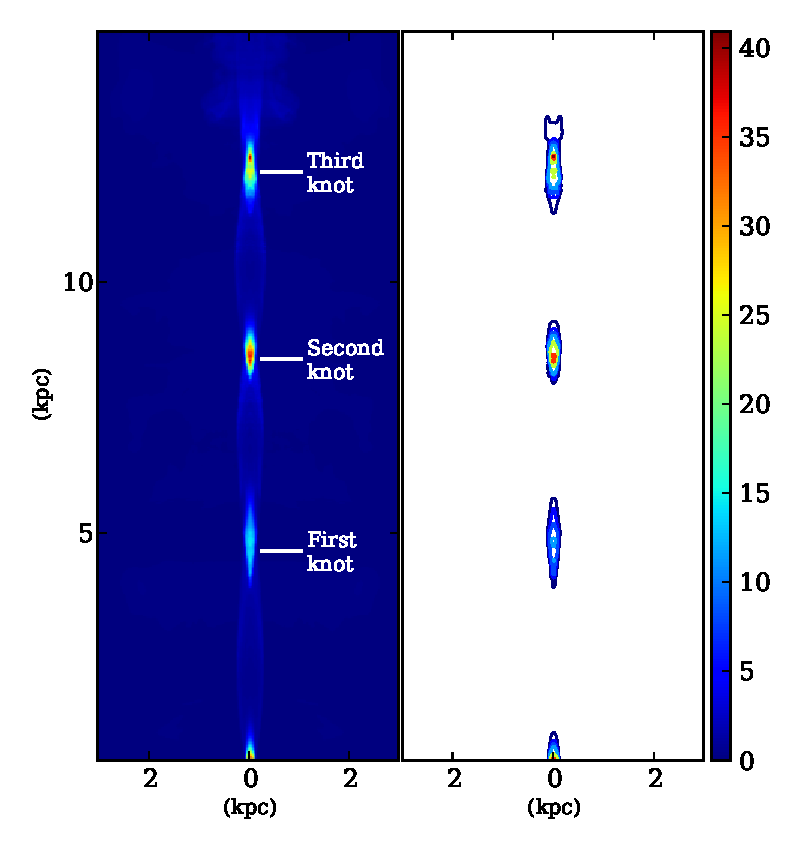
\includegraphics[width=\linewidth]{csb.eps}
\caption{Synthetic surface brightness for model Civ based on an emissivity $j_{\nu} = \delta^{(2+\alpha)} p^{(3+\alpha)/2} \nu^{-\alpha}$, where $\delta= 1/\Gamma(1-\beta \cos 42^\circ)$ is the Doppler factor. The right panel shows the surface brightness contours of the left panel. The contour levels are 4, 8, 11, 14, 25, 35, 40 in arbitrary units.}
\label{radio_morphology}
\end{figure}


To strengthen the association of biconical shocks with the bright knots in the Hydra A northern jet I present a synthetic radio image of one of the best fit models, Ciii, based on an assumed synchrotron emissivity $j_{\nu} \approx {\psi} \, \delta^{2+\alpha} \, p^{(3+\alpha)/2}$, where $\psi$ is the relativistic gas tracer, the Doppler factor $\delta= 1/\Gamma(1-\beta \cos 42^\circ)$ and the pressure dependence assumes that the magnetic pressure is proportional the non-thermal particle pressure \citep[see][\ \S 5.4]{sutherland07a}. Integrated along rays
$I_\nu = \int j_\nu ds$,
 this emissivity provides a semi-quantitative estimate of the surface brightness corresponding to this model.

Fig.~\ref{radio_morphology} (left panel) shows the synthetic surface brightness of the simulated jet. The contour image of the synthetic surface brightness is shown in the right panel. Here I see that, in the shocked zone beyond each biconical shock,  the pressure increases, producing bright knots in each region. This image reproduces some qualitative features of the data: The second and third knots are significantly brighter and more extended than the first knot. However, the 
brightness ratios of the knots are not reproduced. 
Observationally (corrected for resolution) the second knot is 8.7 times brighter than the first and the third knot is 3 times brighter than the second. The model values are 2.5 and 1.14 respectively. In addition, in the observed jet, the FWHM extent of the second knot in the jet direction is 3.3~kpc compared to 0.6~kpc for the model. These differences may possibly be attributed to the approximate magnetic field model, which I have used, or the lack of turbulent three dimensional structure in the simulations. These are aspects to which I can return with three-dimensional simulations with magnetic field. 

%%%%%%%%%%%%%%%%%%%%%%%%%%%%%%%%%%%%%%%%%%%%%%%%%%%%%%%%%%%%%%%%%%%%
%
%		Turbulent Transition
%
%%%%%%%%%%%%%%%%%%%%%%%%%%%%%%%%%%%%%%%%%%%%%%%%%%%%%%%%%%%%%%%%%%%%
\subsection{Transition to turbulence}
\begin{figure*}
\centering
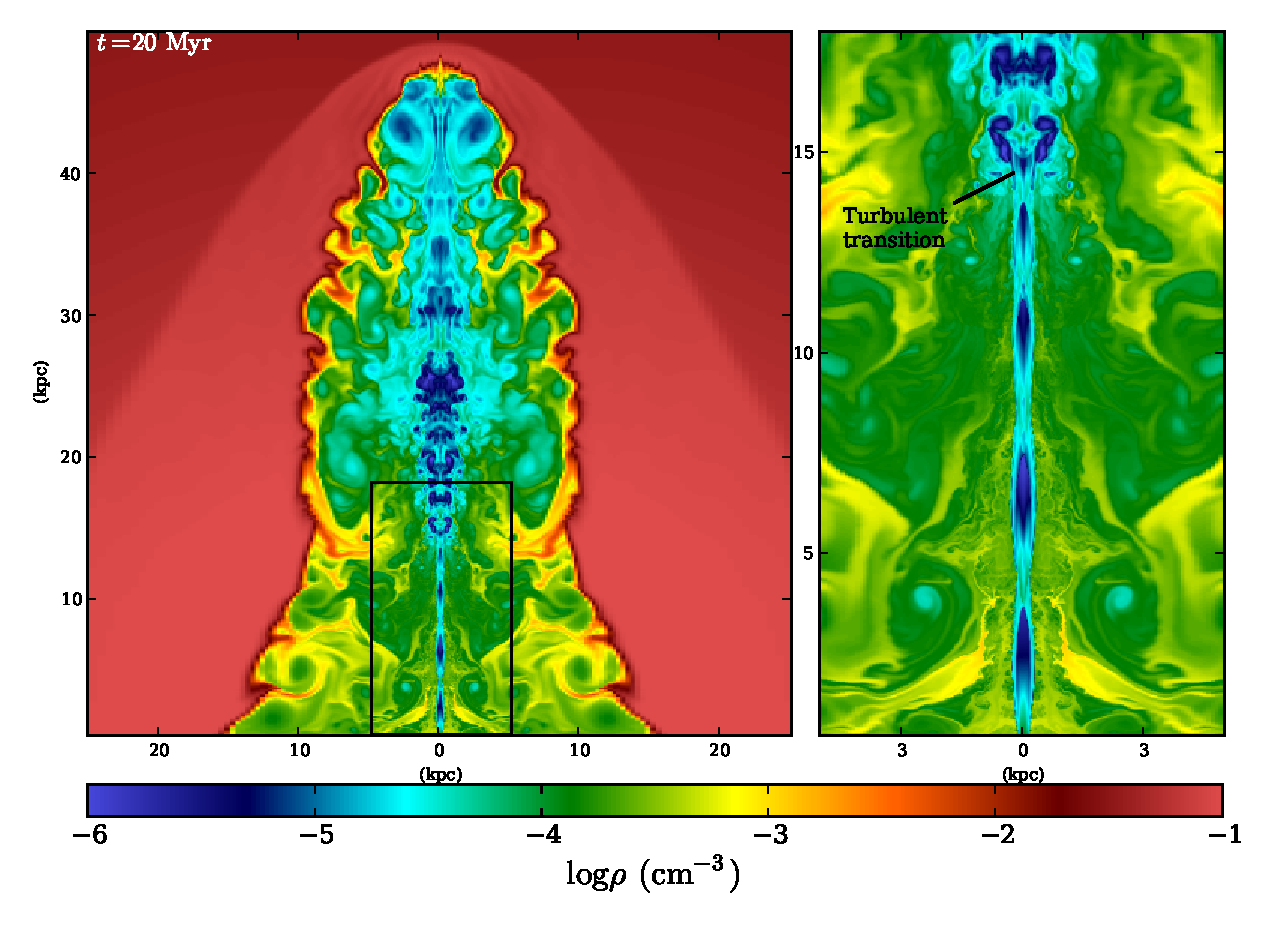
\includegraphics[width=\textwidth]{cbm.eps}
\caption{Logarithmic density snapshot for run Civ at $t=20\,\mathrm{Myr}$ in the left panel. The right panel shows the zoomed in central zone marked with black rectangle in the left panel. This is one of the best fit models, which yields the correct location of the first two biconical reconfinement shocks in the northern jet of Hydra A. A transition to turbulence occurs due to significant shock deceleration of the jet in the reconfinement shocks and the developing Kelvin-Helmholtz instability. }
\label{t_trans}
\end{figure*}
 
 \begin{figure}
\centering
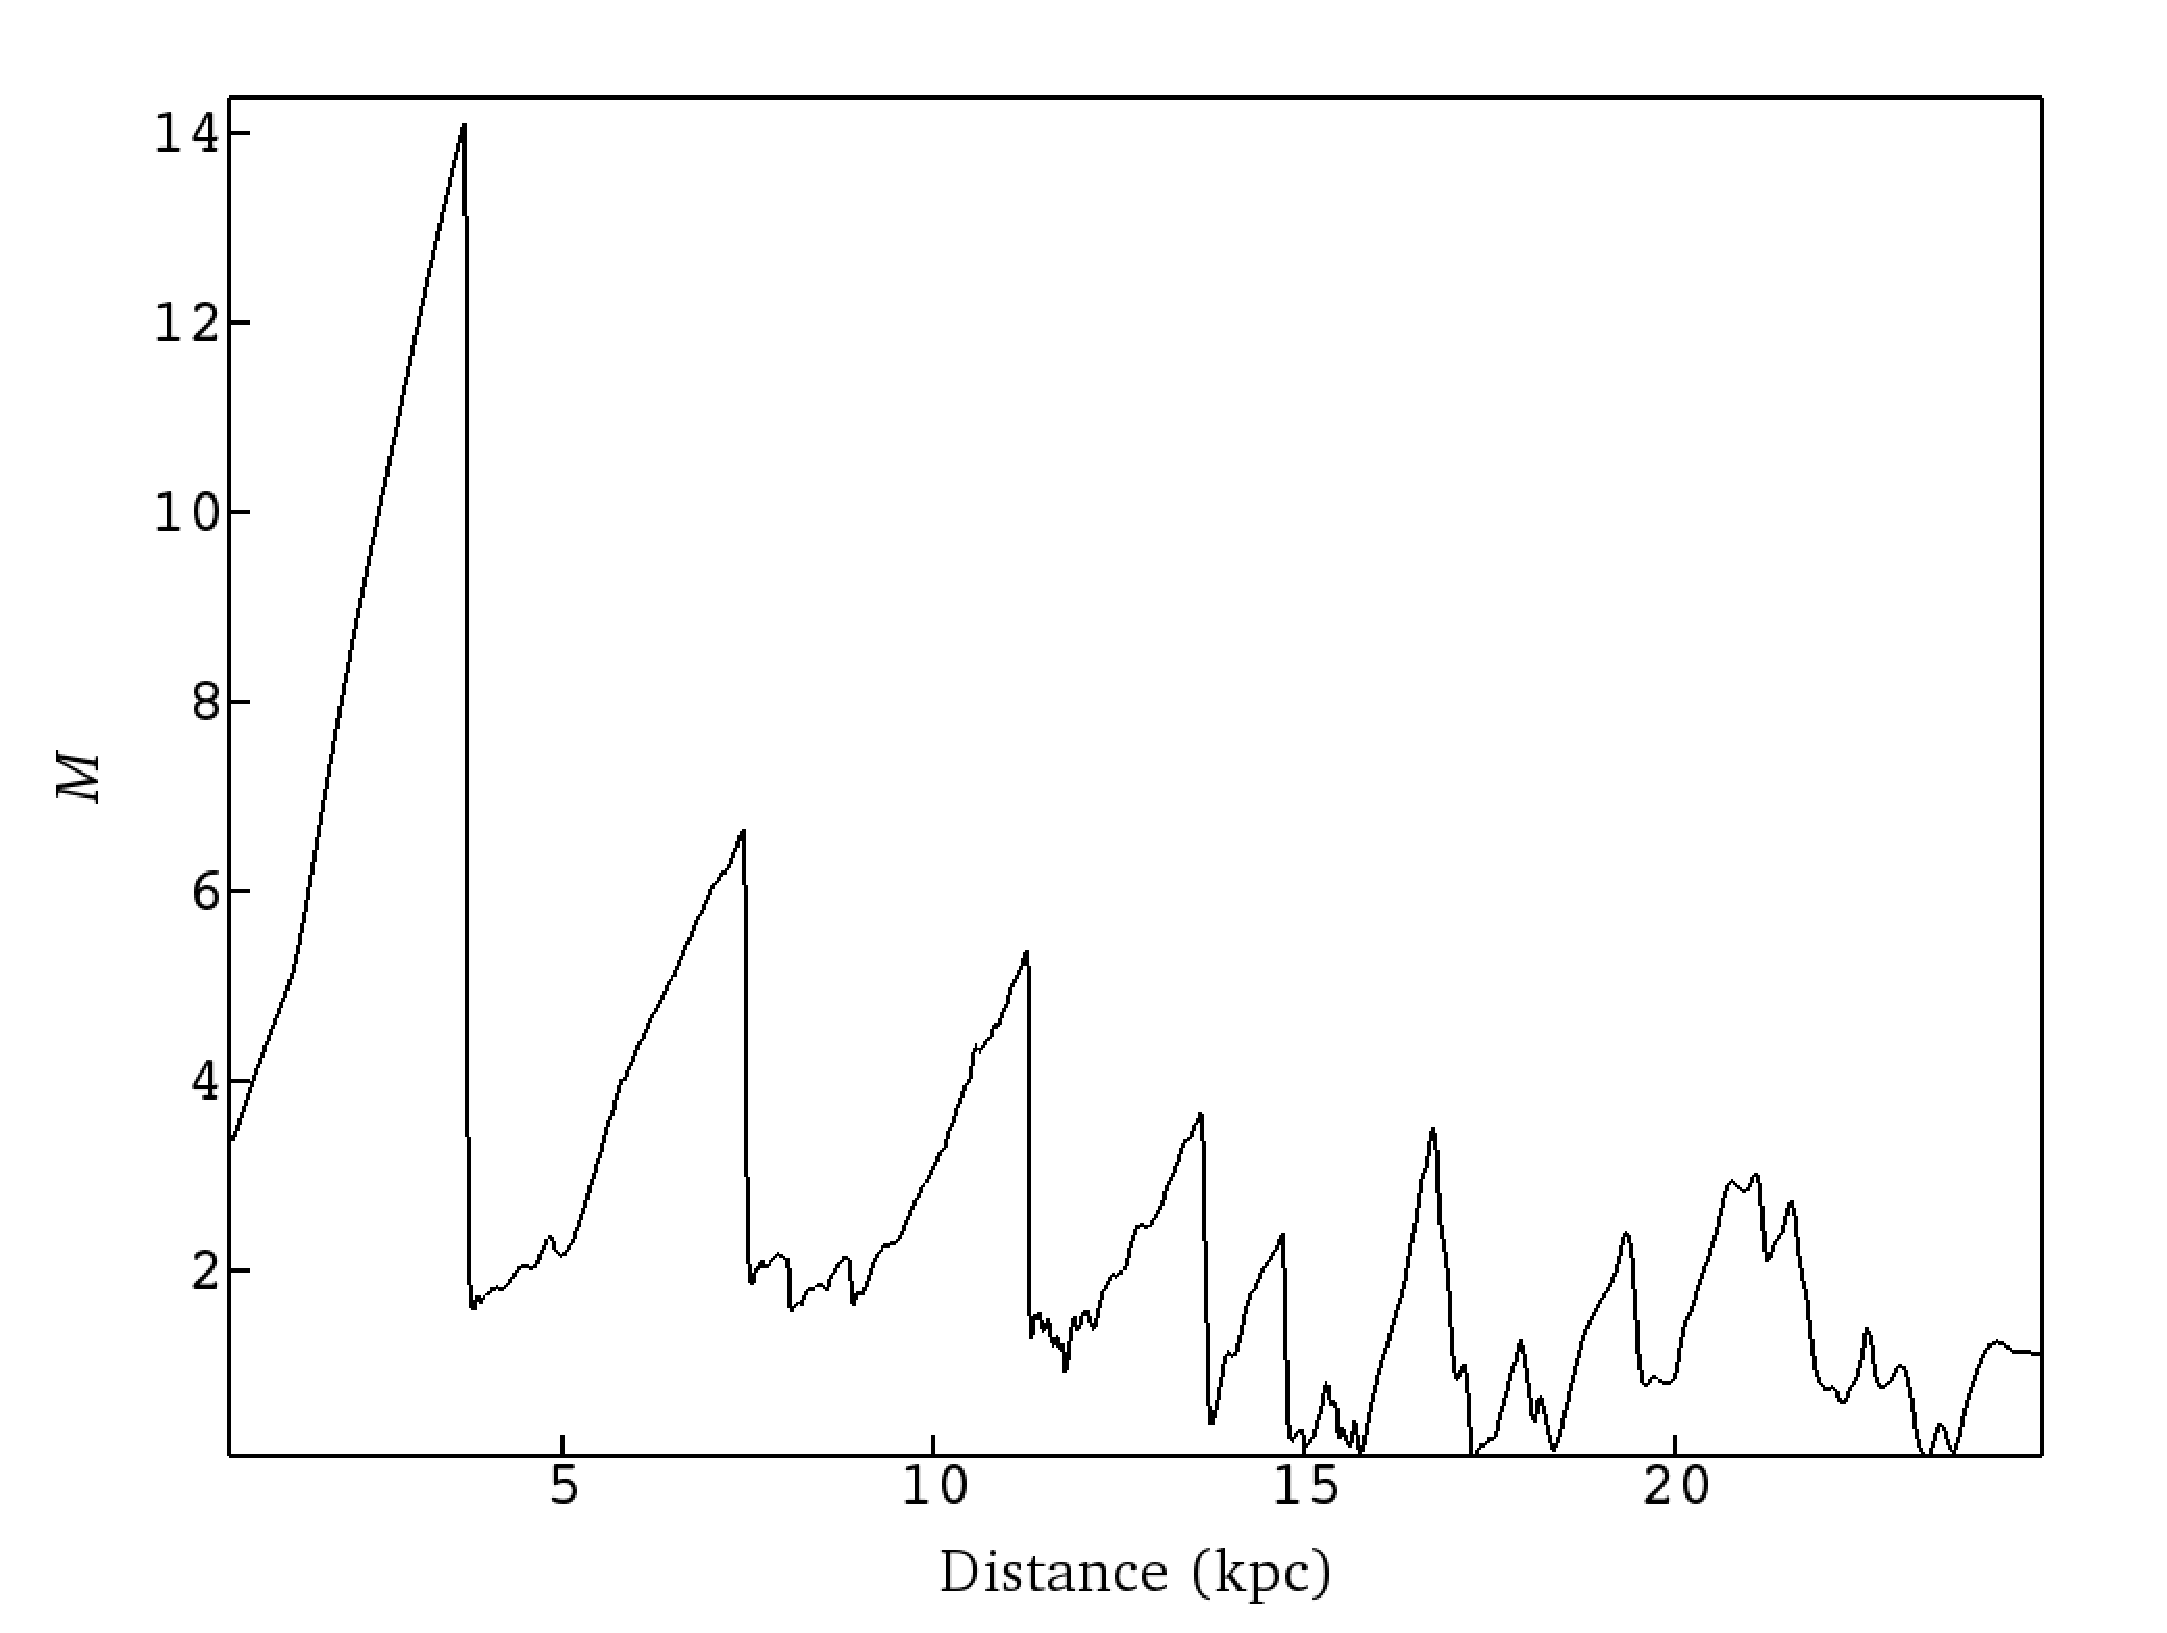
\includegraphics[width=\linewidth]{cml.eps}
\caption{The Mach number of the jet of model Civ at different locations along the jet axis.}
\label{mach}
\end{figure}
 

These two-dimensional models cannot adequately reproduce the structure of the entire source, in particular the plume like regions beyond approximately $7.4^{\prime\prime}$. These are probably the result of three-dimensional turbulence and/or precession, and these effects will be addressed in future study of three dimensional precessing jet model. However, I note that the numerical models \emph{qualitatively} reproduce the turbulent transition of the jets to plumes, albeit at a distance of 14~kpc compared to approximately 11 kpc deprojected in Hydra~A. In the density image snapshot at approximately 20 Myr of run Civ, Fig.~\ref{t_trans} (the left panel shows the full computational domain and the right panel is the zoom in section indicates by the rectangle in the left panel), a series of biconical  shocks appears in the jet.  Deceleration of the jet occurs at these shocks and the jet becomes subsonic after the fourth shock at $\sim 14 \rm \ kpc$ (see the variation of Mach number of the flow with distance along the jet axis in Fig.~\ref{mach}). Beyond 14~kpc the jet transitions to turbulence as a result of the axisymmetric Kelvin-Helmholtz instability, which becomes stronger as the Mach number decreases.) 
Although the axisymmetric jet simulations shed some light on the turbulent transition of the jet, it is well known that turbulence and the formation of plumes are three dimensional phenomena, especially in supersonic flows. I study the details of these features of the inner 20 kpc of the Hydra A jets in the ensuing three dimensional study.


%%%%%%%%%%%%%%%%%%%%%%%%%%%%%%%%%%%%%%%%%%%%%%%%%%%%%%%%%%%%%%%%%%%%
%
%		Brightness Ratio
%
%%%%%%%%%%%%%%%%%%%%%%%%%%%%%%%%%%%%%%%%%%%%%%%%%%%%%%%%%%%%%%%%%%%%

\subsection{Brightness ratio of the jets} \label{s:b_r}
 \begin{figure*}
\centering
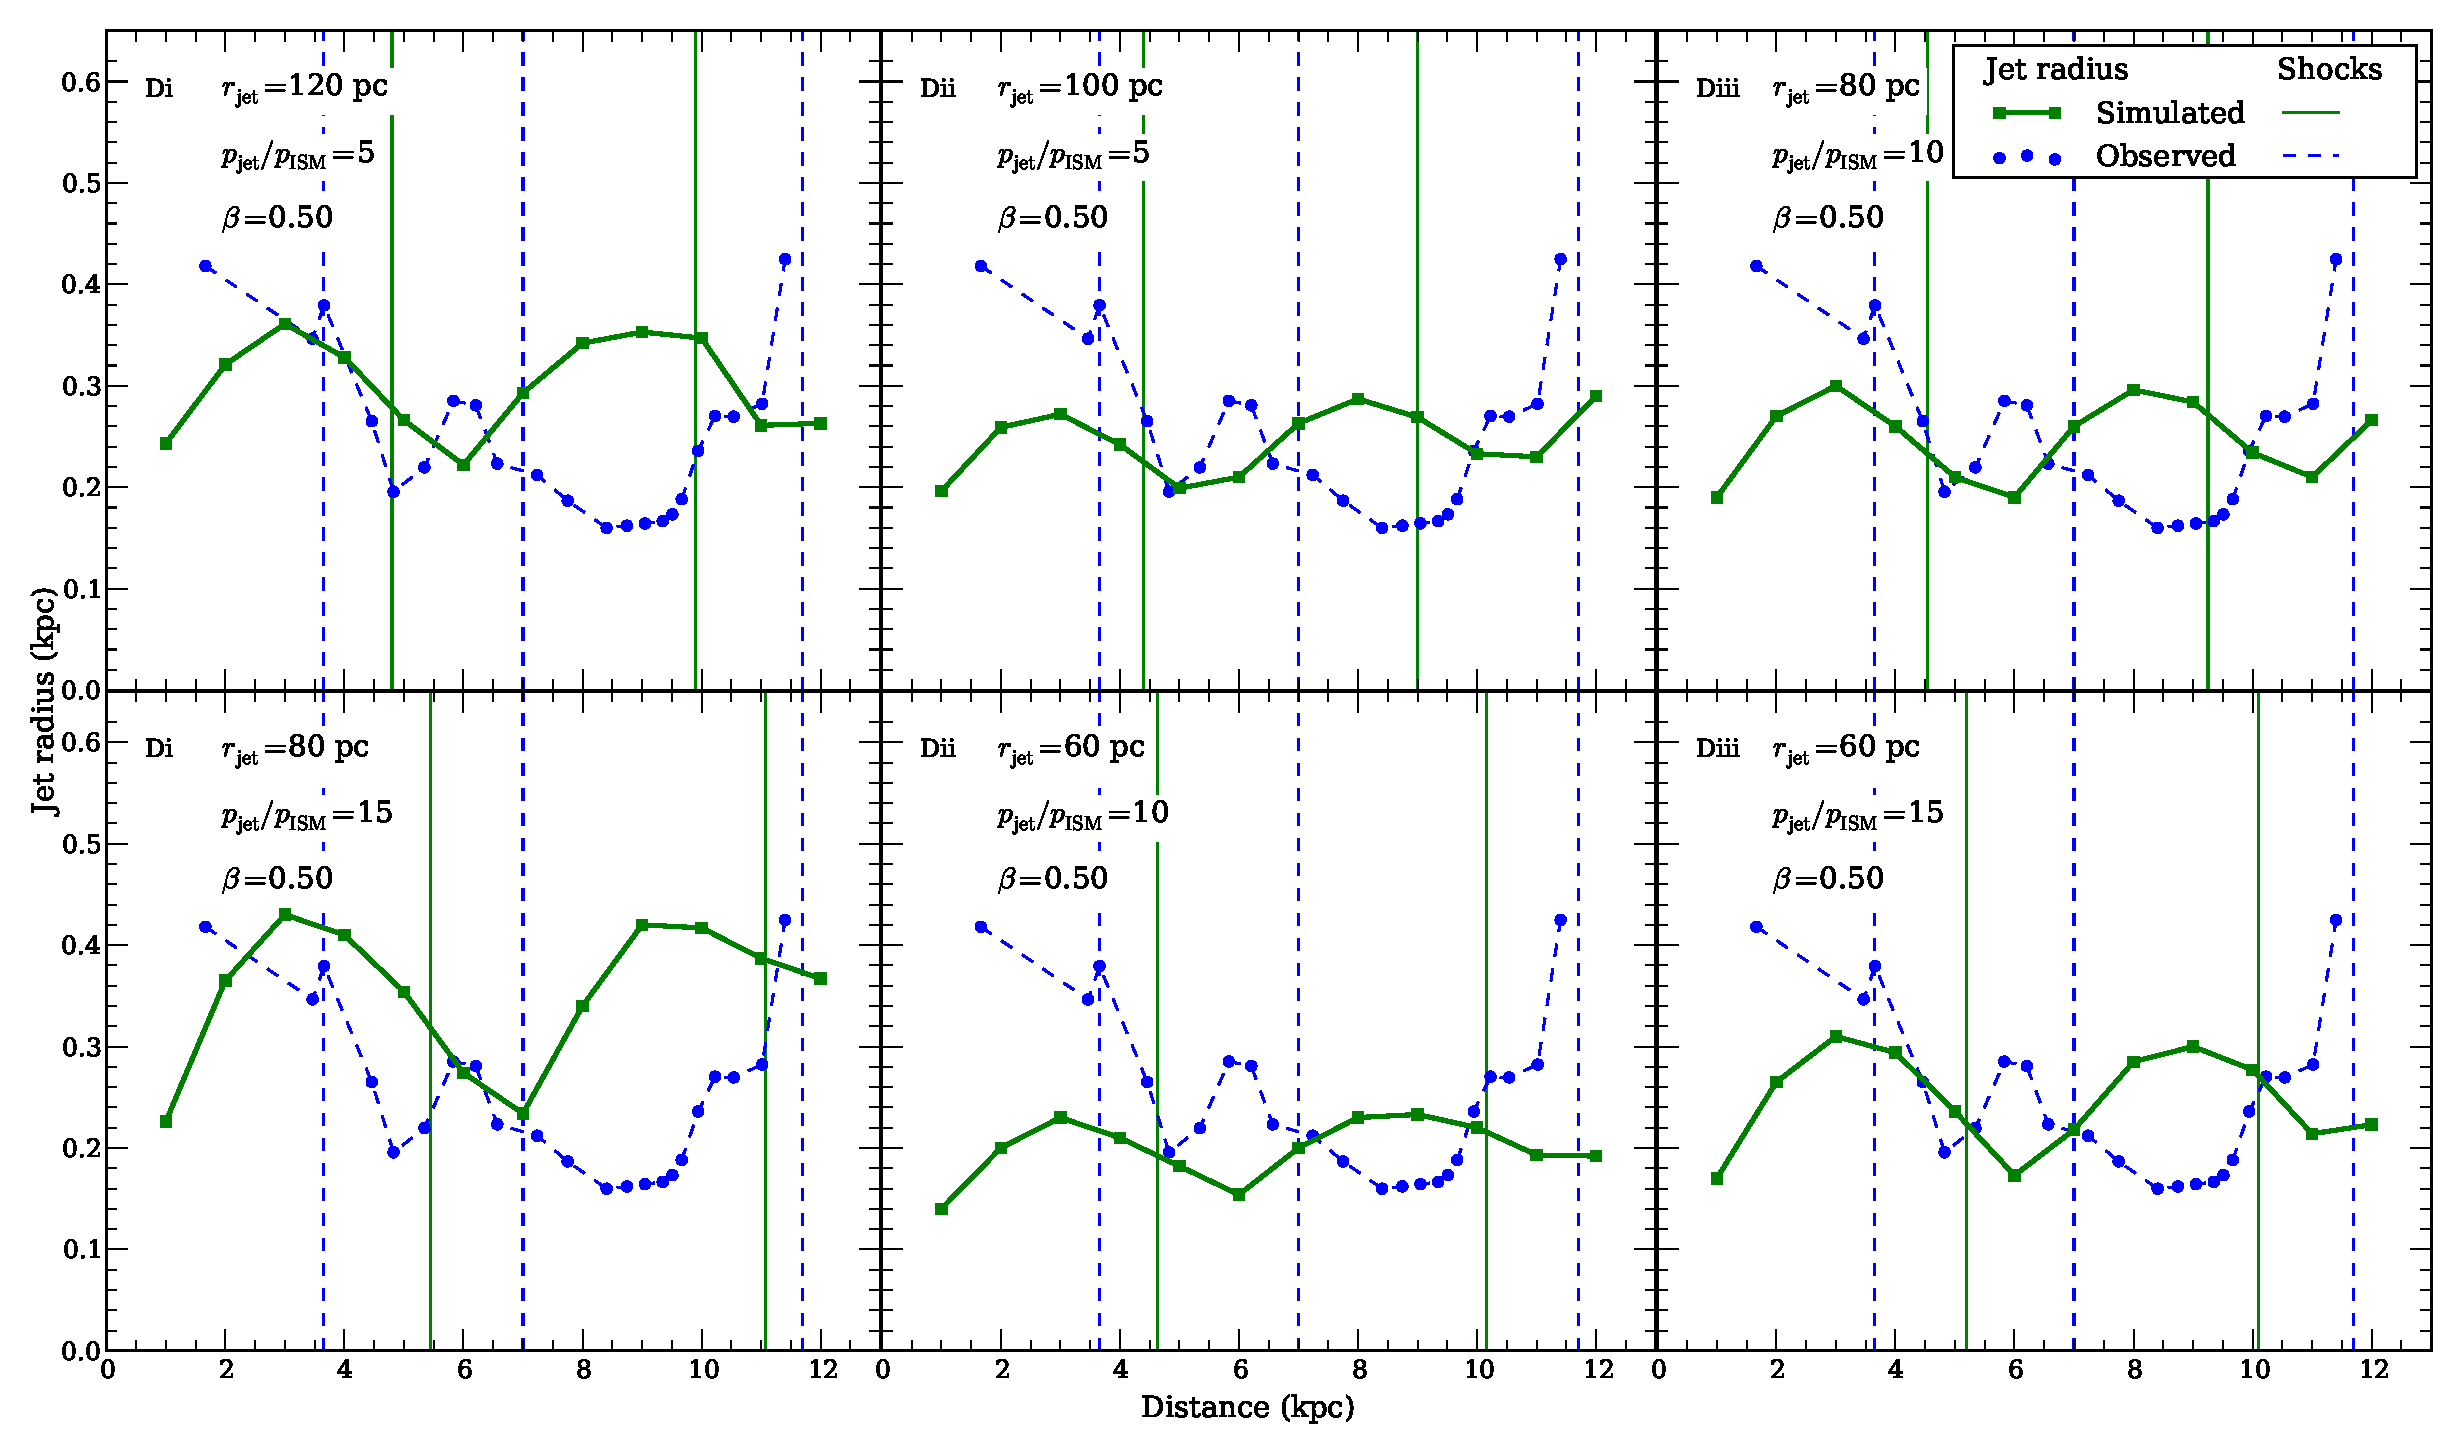
\includegraphics[width=\textwidth]{clv.eps}
\caption{Jet radius profile and shock positions along the jet for jet velocity 0.5. The green line with squares, and the blue lines with circles represent simulated and observation data of radius, respectively. The blue dashed and green solid vertical lines represent the observed and simulated shock locations, respectively.}
\label{f:p_s_b5}
\end{figure*}



I have used the 6cm VLA data of \citet{taylor90} to determine the flux density ratio of the northern and southern jets within the first 10 kpc, obtaining  a value $\approx 7.0$\footnote{\citet{taylor90} quote a value of 1.9, which is close to the observed ratio within 1~kpc.} Attributing this ratio to Doppler beaming, and using the inclination estimated by \citet{taylor90}, implies a moderately relativistic jet  $\beta \approx  0.5$. However, my parameter space study produces a higher jet velocity $\sim 0.8$ which, on the basis of a simple estimate, would give a brightness ratio $\approx 40$. However, in my model, the emissivity is dominated by the decelerated post-shock regions of the jet, so that I estimate the brightness ratio from the synthetic brightness images of approaching and receding jets. With this approach, I obtain a simulated flux density ratio of 33 which still differs significantly from the observed value by a factor $\approx 5$.

I ran several additional models with jet $\beta = 0.5$,  different jet inlet radii 120~pc, 100~pc, 80~pc and 60~pc and different pressure ratio 5, 10, and 15, keeping the jet kinetic power constant at $10^{45} \rm \ ergs \ s^{-1}$. I have not decreased the jet radius below 60~pc because that would require an even more highly over pressured jet to obtain the correct radius profile. These $\beta=0.5$ models are summarised in Table~\ref{t:sim_par} (set D) and the comparison of the simulated and observed shock positions and radius profiles are shown in Fig.~\ref{f:p_s_b5}. It is evident that no model with the given jet kinetic power and jet $\beta = 0.5$ is able to produce good fits for both the shock position and the jet radius. The shock spacings are all significantly larger than the observed shock spacing and the radius profiles are mismatched with these models. 

From the above I can say that if I fix the inclination angle at the \citet{taylor90} value of $42^\circ$ and fix the jet kinetic power at $10^{45} \rm \ ergs \ s^{-1}$, then the jet pressure, jet velocity and the inlet jet radius at 0.5~kpc away from the core of the Hydra A northern jet are well-constrained by both the jet radius profile and the first two knot/shock spacings. The best-fit values are $\beta = 0.75 - 0.85$ and $r_j = 100 \> \rm pc$. Thus, there is a discrepancy in the flux density ratio between the simulated and observed jets. Two potential explanations of the low flux density ratio are: i) Since my models do not include the magnetic field, I employ the assumption $p\propto B^2/8\pi$ which gives a brightness ratio 33. If I further assume that the magnetic field is 2.5 times stronger in the southern jet of Hydra A I would obtain a lower brightness ratio $\sim 7$. ii) The southern jet is more dissipative since it is more twisted and produces more shocks producing a larger intrinsic emissivity than the northern jet. 


%%%%%%%%%%%%%%%%%%%%%%%%%%%%%%%%%%%%%%%%%%%%%%%%%%%%%%%%%%%%%%%%%%%%
%
%		Variation in the inclination angle
%
%%%%%%%%%%%%%%%%%%%%%%%%%%%%%%%%%%%%%%%%%%%%%%%%%%%%%%%%%%%%%%%%%%%%
\subsection{Variation of the inclination angle}\label{s:theta}

 \begin{figure}
\centering
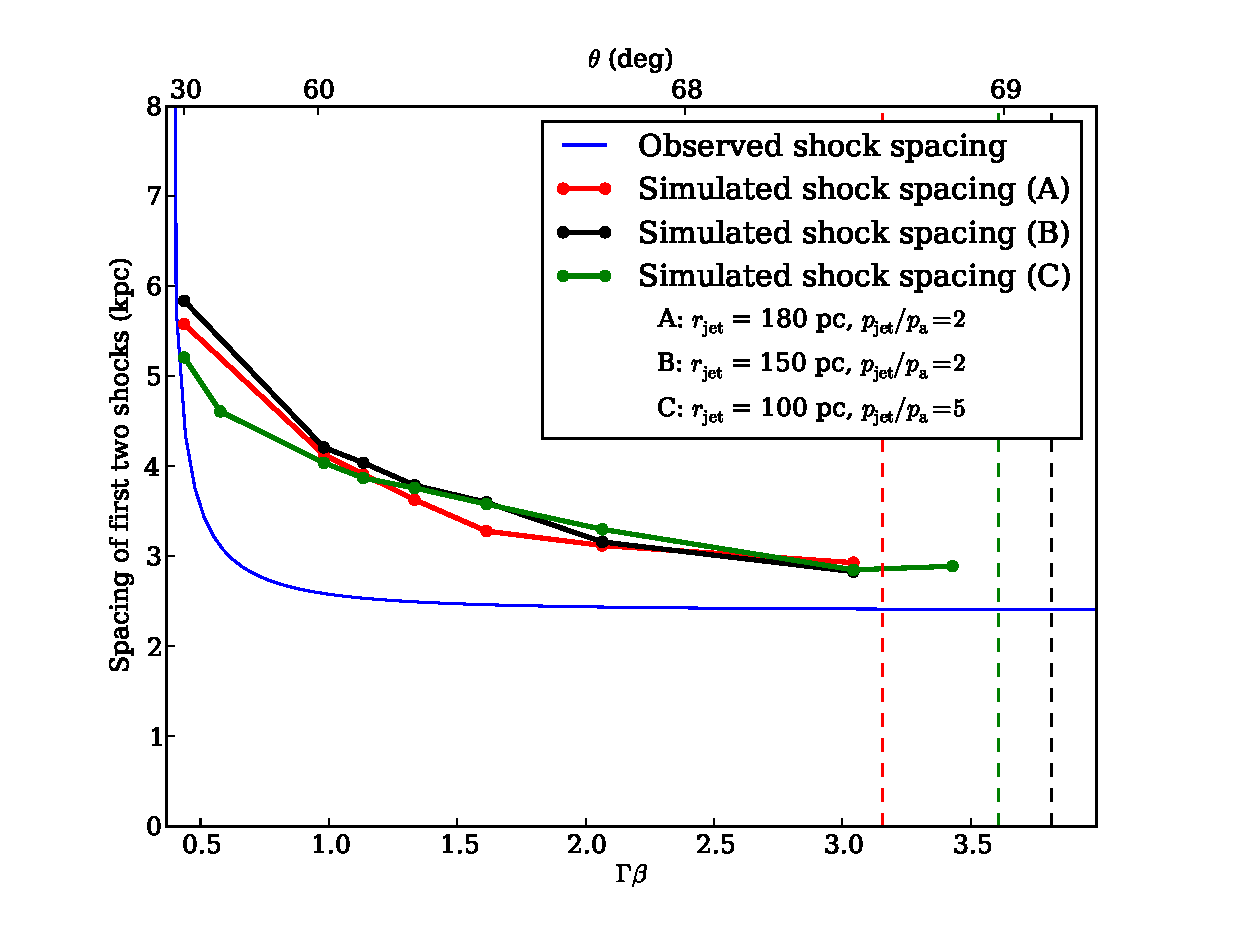
\includegraphics[width=\linewidth]{cts.eps}
\caption{Comparison of the observed  spacing  of the first two shocks (blue curves) with the corresponding simulated shock spacing (red points for model set A, black points for model set B, and green points for model set C) as a function of the 4-velocity $\Gamma \beta$. The dashed vertical lines represent the upper limits of $\Gamma \beta$ for each model (set A -- red, set B -- black, and set C -- green). These limits are estimated for $\chi = 0$ using Eqn.~(\ref{chi2}).}
\label{f:ss}
\end{figure}

In the above models I have used the angle between the jet and the line of sight, $\theta \approx 42^\circ$, estimated by \citet{taylor93} from the rotation measure asymmetry of Hydra~A. However, there is a fairly large uncertainty in their estimate of $\theta$ with $30^\circ \leq \theta \leq 60^\circ$. Increasing $\theta$ from $42^{\circ}$, would reduce the brightness ratio? However, for larger inclinations, the deprojected knot separation would decrease, and as I have seen with the above models, this would require a higher velocity than $0.8 \rm c$, tending to \emph{increase} the brightness ratio. Similar considerations apply if I \emph{decrease} the inclination. Nevertheless, is it possible that notwithstanding opposing effects, an inclination angle within the \citet{taylor90} range, and a jet velocity, can be found that are consistent with the dual constraints of surface brightness ratio and projected knot spacing? 

In order to assess this possibility I adopted the following procedure: For $\beta$ within the range, $0.35 < \beta < 0.98$ (the lower limit being defined by the brightness ratio, $R=7$) I first estimate the value of $\theta$ corresponding to $R = 7$, using the standard Doppler beaming formula, $\theta (\beta)= \beta^{-1}(R^{1/2.7}-1)(R^{1/2.7}+1)^{-1}$. For these values of $\theta(\beta)$ I determine the deprojected spacing between the first two shocks $D_{1,2}(\beta) = 2.25 /\sin \theta(\beta) \> \rm kpc$ given the observed spacing of 2.25~kpc. This is shown, as a function of the 4-velocity, $\Gamma \beta$, as the blue curve in Fig.~\ref{f:ss}. I then compare the observed deprojected knot spacings with the values inferred from the simulations so that in Fig.~\ref{f:ss} the simulated shock spacing, for model sets A, B and C, are also plotted as functions of $\Gamma \beta$. The upper limits on the 4-velocity for each model (estimated from Eqn.~(\ref{chi2})), associated with a zero density parameter, $\chi = 0$, are also shown as dashed vertical lines. 


The first point to note with this comparison is that for most of allowable range of $\beta$ Fig.~\ref{f:ss} shows that the calculated shock spacing exceeds the observed, deprojected value. At the upper end of the $\beta$ range the simulated shock spacings for each model asymptote to $\approx 2.85$ kpc for values of $\Gamma \beta \gtrsim 3$, i.e., $\beta \gtrsim 0.95$. However the asymptote of the observed shock spacing $\approx 2.4$ kpc. Hence, there is an offset of approximately 0.5~kpc between the asymptotes of the simulated and observed shock spacing for $\Gamma \beta \gtrsim 3$.  

At the other end of the allowable range of velocity, $\beta \approx 0.345$ ($\Gamma \beta = 0.368$), it could be inferred that the simulations and observations intersect at approximately this limiting value. However, this is the result of the steepness at $\beta \approx 0.345$ of the (blue) curve representing the observed deprojected shock spacing as a function of 4-velocity, rather than a real physical correspondence between observed and simulated values. It would be fortuitous if the jet initial velocity were to be almost exactly the same as the lower limit on the jet velocity implied by beaming. Hence I reject a solution at this end of the $\beta$ range on the basis of the ``fine-tuning'' that would be involved in accepting it. Another unappealing feature of a low-$\beta$ solution is that the jet would be initially heavy with $\chi \gtrsim 300$. 
As I noted above, observations and modelling of X-ray observations of the lobes of radio galaxies indicate that jets are initially electron-positron in composition \citep{croston05a,croston14} and $\chi \gtrsim 300$ is inconsistent with this. 
 
Another way of looking at the issue of reconciling shock spacing and flux ratios is the following: Consider the simulation points near the upper end of the $\beta$ range in Fig.~\ref{f:ss}, where the discrepancy between the observed jet and simulated jets with $\chi \sim 1$ is the least. By way of example, consider the (green) point in simulation series C with $\beta=0.95$ ($\Gamma \beta = 3.04$). The simulated flux ratio (see \S~\ref{s:b_r}) for this model is 26.5, a factor of 3.8 higher than the observed value. Thus, even for these models there is an implication of intrinsic differences in the northern and southern jet rest-frame emissivities. Moreover, this ratio is not very different from the value of 33 for the $\beta =0.8$, $\theta = 42^\circ$ model considered earlier.

In view of the above, I conclude that, taking into account the modelling of shock spacing, radius evolution and surface brightness ratios, the most likely situation is that of fast, $\beta \gtrsim 0.8$, jets with an intrinsic difference between the rest-frame emissivities of northern and southern jets.

%%%%%%%%%%%%%%%%%%%%%%%%%%%%%%%%%%%%%%%%%%%%%%%%%%%%%%%%%%%%%%%%%%%%%%%%%
%% 
%%												Further implication of axisymmetric model 
%%
%%%%%%%%%%%%%%%%%%%%%%%%%%%%%%%%%%%%%%%%%%%%%%%%%%%%%%%%%%%%%%%%%%%%%%%%%
%\section{A verification of the axisymmetric model: naked jet}
%The simulations of jets propagating into the cluster atmosphere conducted in the previous two chapters typically evolve for 50 kpc, which is the extent of the simulation domain, over a timescale of approximately 20~Myr. While the shock structures in the jet, the turbulent transition of the jet, and global structures, e.g. the turbulent backflows in the cocoon and forward shock of the bubble, are well captured, the simulation time is less than the age of the source. It is possible therefore that the jet is being affected by the backflow within this restricted domain. The purpose of this chapter, therefore, is to ascertain whether the shock positions seen in the simulations are unaffected by the back flow form the head of the jet. To this end I look at the evolution of the shock positions with time, and also perform a simulation of an unbounded jet -- a jet spanning the entire domain and not bounded by a termination shock. This is more representative of conditions in the inner regions of an evolved radio source, such as that of Hydra A. 
%
%%The simulations of jets propagating into the cluster atmosphere conducted above typically evolve to an extent of 50 kpc, as restricted by the simulation domain, over a timescale of approximately 20~Myr. While the shock structures in the jet, the turbulent transition of the jet, and global structures, e.g. the turbulent backflows in the cocoon and forward shock of the bubble, are well captured, the simulation time is less than the age of the source. I therefore need to ascertain whether the shock positions seen in the simulations are likely to approach asymptotic values with time. To this end I look at the evolution of the shock positions with time, and also perform a simulation of an unbounded jet -- a jet spanning the entire domain and not bounded by a termination shock, which is more representative of conditions in the inner regions of an evolved radio source, such as that of Hydra A. 
%
%\subsection{Simulation results} \label{s:jet_stream}
%\begin{figure}
%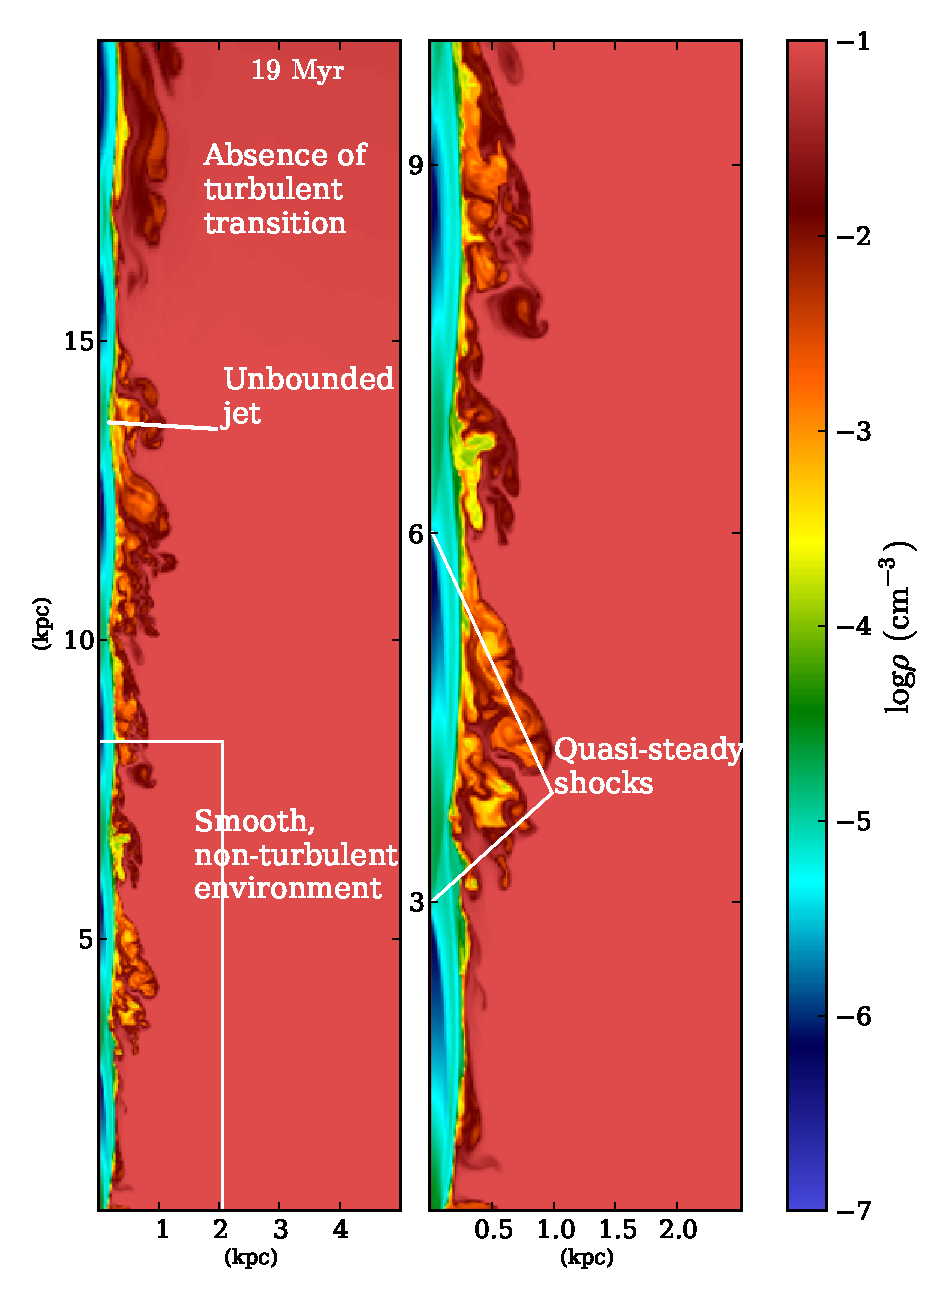
\includegraphics[width=\linewidth]{njm.eps}
%\caption{Logarithmic density image of a simulation of the interaction of an unbounded jet with a non-turbulent ICM. The shock positions are almost time-independent as the jet expands and reconfines multiple times before escaping through the top boundary. No transition to turbulent flow is observed. The right panel is a closeup of the central region marked with a box in the left panel. In both panels the scales are in kpc.}
%\label{f:u_jet}
%\end{figure}
%
%\begin{figure}
%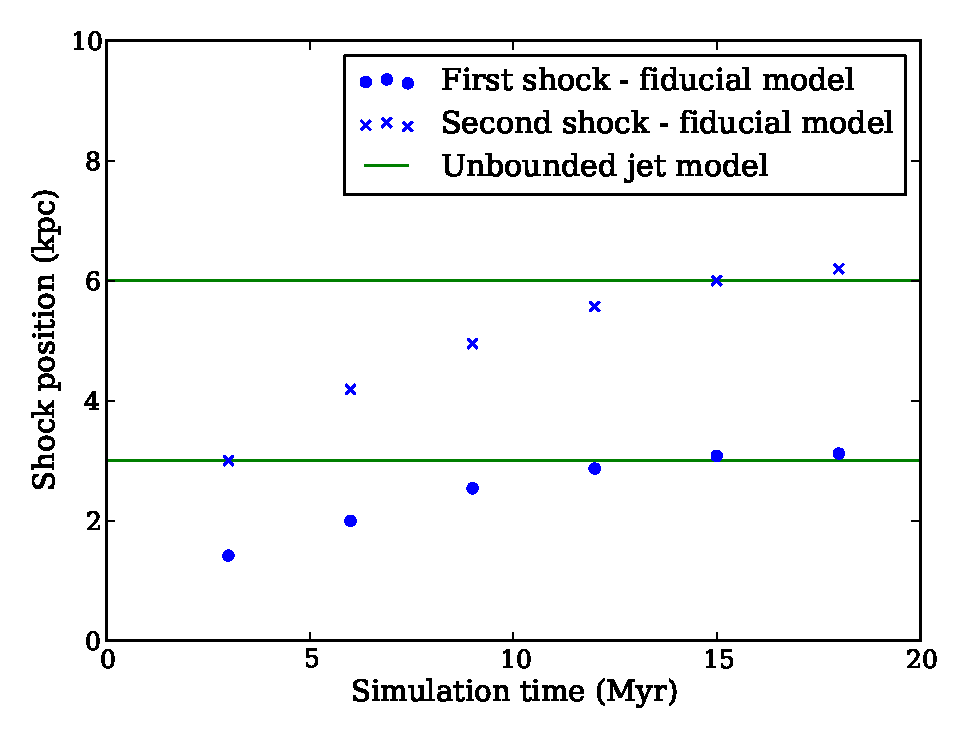
\includegraphics[width=\linewidth]{nse.eps}
%\caption{Evolution of the reconfinement shock positions with time for model Cvii. The circles and crosses represent the first and second shock locations, respectively. The horizontal lines mark the shock positions obtained in the simulation of an unbounded jet using the same parameters as those in model Cvii.}
%\label{f:c_vs_n}
%\end{figure}
%
%Figure~\ref{f:c_vs_n} shows the evolution of the first (circles) and second (crosses) shock positions for model Cv, respectively, as a function of time. The shock positions increase with time, but appear to asymptote to values very close to 3 and 6 kpc, respectively.
%
%In the simulation of an unbounded jet, I set up the the jet inlet with the same jet parameters and geometry as in run Cv, but I also initiate the full extent of a jet column spanning the length of the domain along the jet axis at the start of the simulation. Since the jet is initially overpressured, it expands and contracts, sending a nearly axisymmetric shock wave into the ambient medium, and forming reconfinement shocks along the jet axis. Kelvin-Helmholtz instabilities develop in the shear layer between the jet and the ambient medium, but other than that and the initial adjustment, the flow in the entire simulation box is broadly time-independent. Without a jet backflow, a turbulent cocoon does not develop. Simulations of unbounded jet allow us to measure the quasi-steady reconfinement shock positions because, in the absence of a turbulent cocoon, the global structure of the flow in the simulation domain and the pressure field of the medium surrounding the jet remain fairly steady.
%
%Figure~\ref{f:u_jet} shows the features developed by an unbounded jet model at time $t=19$ Myr. The right panel shows a closeup of the in central $5\times20$ kpc region. The jet is embedded in a relatively steady ambient medium exhibits the first two reconfinement shocks at 3 and 6 kpc. This result is also shown in Fig.~\ref{f:c_vs_n} with two horizontal lines. These shock locations agree with the asymptotic values of the shock position in run Ciii. 
%
%Simulations of unbounded jets are useful for accurately measuring nearly time-independent positions of shocks in a jet, provided the top outflowing boundary is not affecting the structure of the jet. However, these models are not useful in explaining other important features of the Hydra A northern jet, in particular, the turbulent transition of the jet and the formation of the plume structure. As we see in the unbounded jet simulation the deceleration through the biconical shocks and the entrainment in the shear layer alone can not produce the turbulent transition. The ram pressure of the turbulent back flow in the cocoon plays an important role in further deceleration and disruption of the jet, which we see in the simulations of an evolving jet, in which the jet is surrounded by a cocoon of entrained plasma. 
%
%

